\documentclass[titlepage,letterpaper,final,12pt]{scrartcl}

\usepackage[total={6.0in,8.75in},top=1.2in,left=1.35in]{geometry}

% this lets us avoid the scrartcl/hyperref conflict...
%\let\ifvtex\relax

\usepackage{verbatim}
\usepackage{empheq}
\usepackage{color}
\usepackage{animate}
\usepackage{graphicx}
\usepackage{fancyvrb}

% hyperref should be the last package we load
\usepackage[pdftex,
colorlinks=true,
plainpages=false, % only if colorlinks=true
linkcolor=blue,   % only if colorlinks=true
citecolor=blue,   % only if colorlinks=true
urlcolor=blue     % only if colorlinks=true
]{hyperref}

\pdfinfo{
/Title (Numerical modelling of ice sheets, streams, and shelves)
/Author (Ed Bueler)
/Subject (numerical modelling of glaciers, ice sheets, and ice shelves)
/Keywords (numerical modelling, numerical analysis, glacier, ice sheet, ice shelf, shallow models of ice flow)
}

\newcommand{\ddt}[1]{\ensuremath{\frac{\partial #1}{\partial t}}}
\newcommand{\ddx}[1]{\ensuremath{\frac{\partial #1}{\partial x}}}
\newcommand{\ddy}[1]{\ensuremath{\frac{\partial #1}{\partial y}}}
\newcommand{\pp}[2]{\ensuremath{\frac{\partial #1}{\partial #2}}}
\renewcommand{\t}[1]{\texttt{#1}}
\newcommand{\Matlab}{\textsc{Matlab}\xspace}
\newcommand{\bq}{\mathbf{q}}
\newcommand{\bU}{\mathbf{U}}
\newcommand{\eps}{\epsilon}
\newcommand{\grad}{\nabla}
\newcommand{\Div}{\nabla\cdot}
\newcommand{\devstress}{\tau}

\newcommand{\mmess}[1]{\vspace{-0.1in}\begin{center}
\fbox{\url{http://www.dms.uaf.edu/~bueler/mccarthy/mfiles/#1.m}}
\end{center}}

\newcommand{\minput}[1]{
\bigskip
\begin{quote}
\bigskip
\VerbatimInput[frame=single,framesep=3mm,label=\fbox{\normalsize \textsl{\,#1.m\,}},fontfamily=courier,fontsize=\scriptsize]{../mfiles/#1.slim.m}
\bigskip
\end{quote}
}

%\onefig{name}{caption}
\newcommand{\onefig}[2]{
\begin{figure}[ht]
\centering
\includegraphics[width=3.0in,keepaspectratio=true]{#1}
\caption{#2}
\label{fig:#1}
\end{figure}}

%\twofigsizes{left-name}{right-name}{caption}{left-width}{right-width}
\newcommand{\twofigsizes}[5]{
\begin{figure}[ht]
\centering
\includegraphics[width=#4,keepaspectratio=true]{#1} \quad
\includegraphics[width=#5,keepaspectratio=true]{#2}
\caption{#3}
\label{fig:#1}
\end{figure}}

%\twofig{left-name}{right-name}{caption}
\newcommand{\twofig}[3]{\twofigsizes{#1}{#2}{#3}{2.5in}{2.5in}}

\newcommand{\alert}[1]{\emph{#1}}



\begin{document}
\graphicspath{{../photos/}{../pdffigs/}}


\begin{titlepage}

  \begin{center}
    {\Large\usekomafont{title} Numerical modelling \\ of ice sheets, streams, and shelves}
    \vspace{0.5cm}

    {\large Ed Bueler}
    \vspace{1cm}

    September 2012

    \vfill
    
    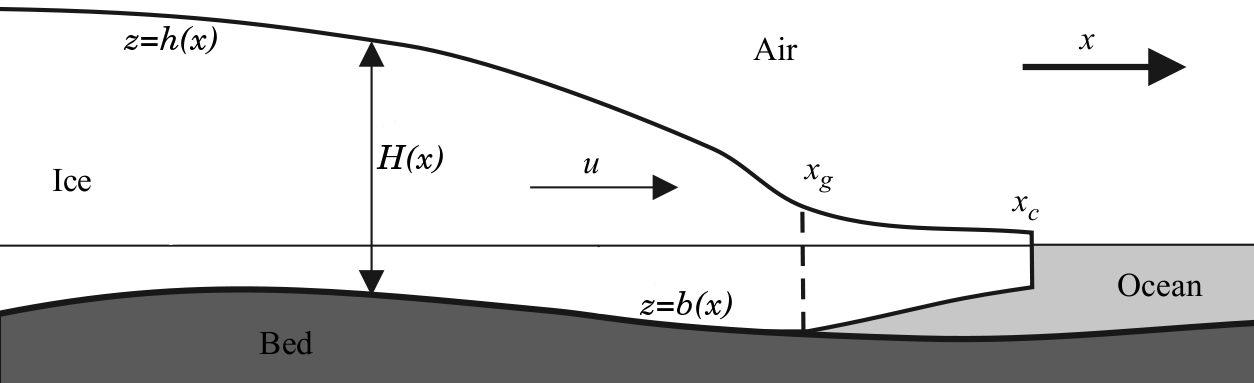
\includegraphics[width=6.0in]{flowline}
  
    \scriptsize \emph{Illustrates the notation used in this chapter.  Figure modified from \cite{SchoofMarine1}.} \normalsize
    
    \vspace{2.0in}
  \end{center}
\end{titlepage}

%\clearpage\newpage
%\tableofcontents

\clearpage\newpage
%\section{Numerical modelling of ice sheets, streams, and shelves}
\setcounter{section}{1}
\subsection{Introduction}

Numerical models can, if well-constructed, actually help understand the behavior of particular glaciers, ice sheets, and ice shelves.  Their most common use may be so that a researcher to ask: when I put together the incomplete understanding of these processes, does the combination behave as I expect, and why does it behave the way I see?  Numerical models rarely generate new theoretical understandings---a human brain seems to be needed to get new insights from observations---but they can surely can demonstrate flaws in the understanding of glacier processes, or in how processes interact to give overall behavior.

But numerical models should be built with care.  The worst outcome is to have a researcher spend time explaining, through physical argumentation and using observational evidence, some model behavior that is simply an artifact of poor computer programming or numerical analysis.  The reader of this chapter may be surprised that the continuum model seems to be much of our focus, but this is because our \emph{intention} to approximate the continuum model requires that we \emph{analyze} the numerical implementation to check that it matches the intent.  All numerical codes produce numbers of some kind, and many produce pretty pictures, but here we want numbers that reflect our intended continuum model.

This chapter has limited goals:
  \begin{enumerate}
  \item we focus on approximating ice flow, and
  \item we provide example numerical codes that actually work.
  \end{enumerate}
But our scope is limited also.  Among the continuum models covered here are the shallow ice approximation (SIA) in two horizontal dimensions (2D), the shallow shelf approximation (SSA) in 1D, and the mass continuity and surface kinematical equations.  We briefly describe the Stokes equations, but we do not address their numerical solution.  The numerical ideas include finite difference schemes, solving algebraic systems from stress balances, and the verification of numerical codes, but we do not use the finite element or spectral methods.

For more on numerical modelling topics not covered here, see the Notes and References section at the end of this chapter.

Our notation generally consistent with the glaciological literature, and other parts of the present book, but Table \ref{tab:notation} gives a summary.  Coordinates are $t,x,y,z$, with $z$ vertical, positive upward.  If the coordinates appear as subscripts then these denote partial derivatives: $u_x = \partial u/\partial x$.  However, tensor notation also uses subscripts from the list $\{1,2,3,i,j\}$, so that $\sigma_{ij}$ is the generic stress tensor entry and $\sigma_{13}$ is a particular entry, for example.
%consistent with \cite{BLKCB,BBssasliding,Fowler,GreveBlatter2009,SchoofStream,SchoofMarine1}

%FIXME: how many codes are displayed?  how many hidden but needed?
This chapter is structured around fourteen Matlab/Octave codes, each of which is about one-half of a page.  These are available in \texttt{.zip} and \texttt{.tar.gz} forms online at:\footnote{Or on a USB drive at Karthaus available from memory stick}

\medskip
  \centerline{\fbox{\url{http://www.dms.uaf.edu/~bueler/karthaus/}}}

\begin{table}% table1, one column
\caption{Common notation used in this chapter.}
\label{tab:notation}
\begin{tabular}{cll}
variable  & description & SI units \\ 
\hline
$A$ & $A=A(T)=$ ice softness in the Glen flow law & $\text{Pa}^{-3}\,\text{s}^{-1}$ \\
$B$ & ice hardness; $B=A^{-1/n}$ & $\text{Pa}\,\text{s}^{1/3}$ \\
$b$ & bedrock elevation & m \\
$g$ & gravity & m s$^{-2}$ \\
$H$ & ice thickness & m \\
$h$ & ice surface elevation & m \\
$M$ & climatic mass balance & m a$^{-1}$ \\
$n$ & exponent in Glen flow law & \\
$p$ & pressure & Pa \\
$\rho$ & density of ice & kg m$^{-3}$ \\
$\rho_w$ & density of sea water & kg m$^{-3}$ \\
$T$ & temperature & K \\
$\tau$ & magnitude of $\tau_{ij}$: \quad $2 \tau^2 = \sum_{ij} \tau_{ij}^2$ & Pa \\
$\tau_{ij}$ & deviatoric stress tensor & Pa \\
$Du_{ij}$ & strain rate tensor & s$^{-1}$ \\
$\mathbf{u}$ & $=(u,v,w)$ ice velocity & m s$^{-1}$ \\
\end{tabular}
\end{table}

\subsubsection*{Ice flow equations}  My first goal in these notes is to get to an equation for which I can say:
\begin{center}
\emph{numerically solve just this equation, and you've got a usable model for a flowing ice sheet.}
\end{center}
Note that a ``usable'' model is \emph{understood} more than it is \emph{correct}!

To get to my goal I will quickly recall the continuum mechanics of ice flow.  Ice in glaciers is a \emph{fluid}.  Thus we describe fluids primarily by a \emph{velocity field} $\mathbf{u}(t,x,y,z)$.  If the ice fluid were either faster-moving than it actually is (e.g., because gravity was much stronger), or if it was linearly-viscous like liquid water (with a viscosity $\nu$), or both, then ice flow would be a more-familiar, ``typical'' fluid.  We would use the Navier-Stokes equations as our flow model:
\begin{align}
\nabla \cdot \mathbf{u} &= 0 &&\text{\emph{incompressibility}} \label{incompressible} \\
\rho \left(\mathbf{u}_t + \mathbf{u}\cdot\nabla \mathbf{u}\right) &= -\nabla p + \nu \nabla^2 \mathbf{u} + \rho \mathbf{g} &&\text{\emph{stress balance}} \label{navierstokes}
\end{align}
Equation \eqref{navierstokes} says essentially ``$ma=F$'', as in Newton's second law.  In \eqref{navierstokes} the term in parentheses is an acceleration and the right-hand side is the total stress.

You say ``\emph{hmmm} \dots \emph{does not sound like glaciology to me!}''  Indeed, is numerical ice flow modeling a part of computational fluid dynamics?  My answer is emphatically ``yes''.  It is a large scale fluid problem like atmosphere and ocean modelling in climate systems.  But it is a weird one!  Consider the kinds of topics which make atmosphere and ocean flow modelling exciting:
  \begin{center} turbulence \qquad convection \qquad  coriolis force  \qquad salinity \qquad chemistry
  \end{center}
None of this topic list is relevant to ice flow.  So what could be interesting about the flow of slow, cold, stiff, laminar, inert old ice?  Of course, it is \emph{ice dynamics!}

We observe that ice is a slow, shear-thinning fluid.  In terms of equations, ``slow'' implies that $\rho \left(\mathbf{u}_t + \mathbf{u}\cdot\nabla \mathbf{u}\right) \approx 0$, which is to say that the forces of inertia are negligible.  And glaciers have shear-thinning flow---a specific ``non-Newtonian'' behavior.  Bigger strain rate means smaller viscosity.  Thus the viscosity $\nu$ in \eqref{navierstokes} is not constant, and we replace this constant viscosity by a ``flow law'', the famous Glen law.

Thus the standard ``full'' model for isothermal flow is the set of Stokes equations:
\begin{align}
\nabla \cdot \mathbf{u} &= 0 &&\text{\emph{incompressibility}} \label{incompressibleagain} \\
0 &= - \nabla p + \nabla \cdot \tau_{ij} + \rho \mathbf{g} &&\text{\emph{stress balance}} \label{forcebalance} \\
Du_{ij} &= A \tau^2 \tau_{ij} &&\text{\emph{$n$=3 Glen flow law}} \label{flowlaw}
\end{align}
In the flow law, the deviatoric stress tensor $\tau_{ij}$ and the strain rate tensor $Du_{ij}$ appear; previous lectures on continuum mechanics cover these.  The facts about these tensors which we need here are that each has trace zero and also that $2\,Du_{ij} = (u_i)_{x_j}+(u_j)_{x_i}$.

The Stokes equations are true at every instant.  Therefore geometry, boundary stresses, and ice softness together determine the velocity field instantaneously.  In fact, a time-stepping numerical ice sheet code recomputes the full velocity field at every time step.  The code does not need the velocity from the previous step---ice flow models have no memory of momentum.  Velocity is a ``diagnostic'' output.


\subsubsection*{Slab-on-a-slope}  Consider now the  $x,z$ plane flow case, so that $v=0$ and all derivatives with respect to $y$ are zero.  The Stokes equations then say
\begin{empheq}[]{align}
u_x + w_z &= 0 &&\text{\emph{incompressibility}} \label{incompressiblexz} \\
p_x &= \tau_{11,x} + \tau_{13,z} &&\text{\emph{stress balance} ($x$)} \label{stokespx} \\
p_z &= \tau_{13,x} - \tau_{11,z} - \rho g &&\text{\emph{stress balance} ($z$)} \label{stokespz} \\
u_x &= A \tau^2 \tau_{11} &&\text{\emph{flow law} (diagonal)}  \label{forceflowx} \\
u_z + w _x &= 2 A \tau^2 \tau_{13} &&\text{\emph{flow law} (off-diagonal)} \label{forceflowz}
\end{empheq}
Here $x,z$ subscripts are partial derivatives.  Note that $\tau_{13}$ is a ``vertical'' shear stress while $\tau_{11}$ and $\tau_{33}=-\tau_{11}$ are deviatoric longitudinal stresses.

We have five equations in five unknowns ($u,w,p,\tau_{11},\tau_{13}$).  This is complicated enough to make many researchers pause before jumping in to a solution method.  Can we first handle a simplified situation?  Our first example is both a case in which we actually solve the Stokes equations, and a primary example to motivate the shallow model which follows.  We will only use rotated coordinates in this first example, and not elsewhere in these notes.

\onefig{slab}{FIXME: $\alpha$ not $\theta$  Configuration of slab-on-a-slope flow calculation.}

Consider the two-dimensional axes ($x$,$z$) show in Figure \ref{fig:slab}, which are rotated downward at angle $\alpha>0$ so that the gravity vector has components $\mathbf{g} = (g \sin\alpha,- g \cos \alpha)$.  Equations \eqref{stokespx}, \eqref{stokespz}, in rotated coordinates, are now:
\begin{align}
p_x &= \tau_{11,x} + \tau_{13,z} + \rho g \sin\alpha, \label{stokespxrot} \\
p_z &= \tau_{13,x} - \tau_{11,z} - \rho g \cos\alpha. \label{stokespzrot}
\end{align}

In a slab-on-a-slope we suppose there is no variation in $x$.  Thus the whole set of Stokes Equations \eqref{incompressiblexz}, \eqref{forceflowx}, \eqref{forceflowz}, \eqref{stokespxrot}, \eqref{stokespzrot} simplify:
\begin{align}
w_z &= 0 &   0 &= \tau_{11} \label{slabblock} \\
\tau_{13,z} &= - \rho g \sin\theta &   u_z &= 2 A \tau^2 \tau_{13} \notag \\
p_z &= - \rho g \cos\theta \notag
\end{align}
We apply boundary conditions:
	$$w(\text{base})=0, \qquad p(\text{surface})=0, \qquad u(\text{base})=u_0,$$
where the basal velocity $u_0$ will remain undetermined for now.  By integrating vertically, we get $w=0$, $p = \rho g \cos\theta (H-z)$, and a linear increase with depth for the shear stress,
	$$\tau_{13} = \rho g \sin\theta (H-z)$$
From \eqref{forceflowz} and $w_x=0$ we also get a formula for the horizontal velocity,
\begin{align}
u(z) &= u_0 + 2 A (\rho g \sin\theta)^3 \int_0^z (H-z')^3\,dz' \label{uslab} \\
     &= u_0 + \frac{1}{2} A (\rho g \sin\theta)^3  \left(H^4 - (H-z)^4\right) \notag
\end{align}

Do we believe these equations?  Figure \ref{fig:slabvel} compares the velocity from equation \eqref{uslab} to observations of a mountain glacier.  We have done a credible job of capturing the deformation flow velocity, but we do not yet have a model for the sliding velocity $u_0$.  

\twofigsizes{slabvel}{athabasca_deform}{Left: velocity from the slab-on-a-slope example calculation.  Right: velocity measured in a mountain glacier, the Athabasca Glacier in Canada, derived from inclinometry \cite{SavagePaterson}.}{2.4in}{2.0in}

Now that we have calculated the velocity $u=u(t,x,z)$ \dots so what?  The equations so far do not address the change in shape of the glacier or ice sheet.  So we consider another equation, the \emph{mass continuity} equation.  To explain this, suppose our slab has variable thickness $H=H(t,x)$ and define the vertical average of velocity:
	$$\bar u(x,t) = \frac{1}{H}\int_0^{H} u(t,x,z)\,dz.$$
The product $\bar u\, H$ is the rate of flow input into the side of the area in Figure \ref{fig:slabmasscontfig}.

Now, how does the ice area $A$ in the figure change?\footnote{In three-dimensions it would be ``How does the ice volume change?''}  We compute
	$$\frac{dA}{dt} = \int_{x_1}^{x_2} M(x)\,dx + \bar u_1 H_1 - \bar u_2 H_2$$
If the width $dx=x_2-x_2$ is small then $A\approx dx\, H$.  So we divide by $dx$ and get
\begin{equation}
H_t = M - \left(\bar u H\right)_x \label{masscont1D}
\end{equation}
This mass continuity equation describes the change in the ice thickness in terms of surface mass balance and also the ice velocity.

\onefig{slabmasscontfig}{The mass continuity equation \eqref{masscont1D} follows from considering the changing area of ice $A$ in a flow line.  Ice can be added at the top by mass balance $M$.  A difference of flow into left and right sides can also change the area.}


\subsection{Shallow ice sheets}  Our slab-on-a-slope example now gives us a rough explanation of the shallow ice approximation (SIA) which we will use more generally.  From the slab-on-slope velocity formula \eqref{uslab} in the $u_0=0$ case (non-sliding case) we get
\begin{align*}
\bar u H &= \int_0^H \frac{1}{2} A (\rho g \sin\theta)^3  \left(H^4 - (H-z)^4\right)\,dz \\
	&= \frac{1}{2} A (\rho g \sin\theta)^3  \left(\frac{4}{5} H^5\right) \\
	&= \frac{2}{5} A (\rho g \sin\theta)^3 H^5
\end{align*}
Note that $\sin \theta \approx \tan\theta = - h_x$.  Combining these with mass continuity \eqref{masscont1D} gives
\begin{equation}
  H_t = M + \left(\frac{2}{5} (\rho g)^3 A H^5 |h_x|^2 h_x\right)_x. \label{sia1D}
\end{equation}
This equation is ``the'' SIA equation.  Note $h=H+b$.  Equation \eqref{sia1D} determines the evolution of ice sheets in terms of mass balance, ice softness, and bed elevation.

Additional arguments are needed to actually show that the SIA is ``general purpose'' and not special to a simple slab.  See Notes and References for these general arguments.  They derive the SIA model from the Stokes equations, under the assumption that slopes and the depth-to-width ratio are small.

We will numerically solve the SIA equation in section \ref{sec:numericalsia}.  First we seek to understand it a bit better, and state it in two horizontal dimensions.

\subsubsection*{Understanding the shallow ice approx (SIA)}  Ice sheets have four outstanding properties as fluids.  They are (\emph{i}) slow, (\emph{ii}) shallow,  (\emph{iii}) non-Newtonian, and (\emph{iv}) they sometimes experience contact slip.  Regarding ``shallow'', Figure \ref{fig:green_transect} shows a no-vertical-exaggeration version of a cross section of Greenland at $71^\circ$.  The vertically-exaggerated shape also shown in the Figure is far more familiar in the glaciological literature, but remember that these flows are thin.

\onefig{green_transect}{The standard vertically-exaggerated cross section of the Greenland ice sheet $71^\circ$ north latitude is shown by the vertical axis labels, and the green and blue curves.  The version without such exaggeration is in red.}

The first ice flow model we consider is the non-sliding, isothermal shallow ice approximation or ``SIA'' for short.  It applies to small depth-to-width ratio (``shallow'') grounded ice sheets on not-too-rough bed topography, whose flow is not dominated by sliding and/or liquid water at the base or margin.

The SIA uses the formulas from slab-on-a-slope, generalized to two horizontal dimensions.  Let $\mathbf{u} = (u,v)$ be the vector horizontal velocity.  The SIA has a shear stress approximation
	$$(\tau_{13},\tau_{23}) \approx - \rho g (h-z) \nabla h.$$
From Equation \eqref{flowlaw}, and further approximation of the shear strain rates in planes parallel to the geoid, we get a formula for a strain rate,
\begin{align*}
\mathbf{u}_z &\approx 2 A |(\tau_{13},\tau_{23})|^{n-1} (\tau_{13},\tau_{23}) \\
     &= - 2 A (\rho g)^n (h-z)^n |\nabla h|^{n-1} \nabla h.
\end{align*}
By integrating vertically, in the non-sliding case, we get
\begin{equation}
\mathbf{u} = - \frac{2 A (\rho g)^n}{n+1} \left[H^{n+1} - (h-z)^{n+1}\right] |\nabla h|^{n-1} \nabla h.  \label{siavelocity}
\end{equation}

Mass continuity in two horizontal dimensions also applies:
\begin{equation}
    H_t = M - \Div\left(\bar{\mathbf{u}} H\right)  \label{masscont}
\end{equation}
Compare Equation \eqref{masscont1D} in one dimension.

Combining Equations \eqref{siavelocity} and \eqref{masscont} and defining a positive constant $\Gamma = 2 A (\rho g)^n / (n+2)$, we get an equation for the rate of thickness change in terms of mass balance $M$, thickness, and surface slope $\grad h$:
\begin{equation}
H_t = M + \Div \left(\Gamma H^{n+2} |\grad h|^{n-1} \grad h \right) \label{sia}
\end{equation}

Fulfilling an earlier promise, if we just solve \eqref{sia} numerically then we get a usable model for the Barnes ice cap, see for example \cite{Mahaffy}.  The Barnes ice cap is a particularly simple ice sheet on a very flat bed with minimal evidence for sliding.


\subsubsection*{Analogy with the heat equation}  An obligatory step in using the SIA model is realizing that Equation \eqref{sia} is analogous to the better known heat equation.  All numerical methods for solving \eqref{sia} can be understood as modifications of well-known heat equation methods.

Recall first that the heat equation comes from simple empirical observations like Newton's law of cooling, the ordinary differential equation
	$$\frac{dT}{dt} = -K (T-T_{\text{ambient}})$$
where $T$ is object temperature and $K$ relates to material and geometric properties of an object (e.g.~a cup of coffee).  That is, the temperature of an object tends to decay exponentially to the temperature of its surroundings (ambient temperature $T_{\text{ambient}}$).  One way to derive the heat equation, which is a partial differential equation, is to argue that the segments of a rod also satisfy Newton's law of cooling.  Segment $j$ with temperature $T_j$ sees an ambient temperature which is the average temperature of the segment's neighbors:
   $$\frac{dT_j}{dt} = -K \left(T_j - \frac{1}{2} (T_{j-1} + T_{j+1}) \right) = \frac{K}{2} \left(T_{j-1} - 2 T_j + T_{j+1}\right).$$
As segment lengths shrink to zero we see an approximation of the second derivative with respect to $x$ on the right, because $K$ scales with $\Delta x^2$, the square of the segment length.  Thus the distributed temperature of a rod satisfies
\begin{equation}
  T_t = D T_{xx}. \label{heat1D}
\end{equation}
This is the one dimensional heat equation when material properties are constant.  The constant $D$ is the ``diffusivity''.

The more complete 2D version of the heat equation describes the temperature $T(t,x,y)$ at position $x,y$ in an object and at time $t$.  Fourier's law and conservation of energy replace the above ad hoc Newton's law of cooling argument.  Fourier's law is a rule for heat flux, namely $\mathbf{q} = - k \grad T$.  If we allow an additional heat source $f$, conservation of energy says $\rho c T_t = f - \Div \mathbf{q}$.  Combining these we get the standard heat equation:
	$$\rho c T_t = f + \Div (k \grad T).$$
Here $\rho$ is density, $c$ is specific heat, and $k$ is conductivity.  Now define the ``diffusivity constant'' $D=k/(\rho c)$ and also $F = f/(\rho c)$.  Then the heat equation is
\begin{equation}
T_t = F + \Div (D\, \grad T). \label{heat}
\end{equation}
Figure \ref{fig:initialheat} shows a solution of the heat equation, where the initial condition is a localized ``hot spot''.  Solutions of the heat equation involve the spreading, in all directions, of local heat maxima, that is, diffusion.

\twofigsizes{initialheat}{finalheat}{Left: Initial condition $T(0,x,y)$.   Right: Solution $T(t,x,y)$ at $t=0.02$.  (The right picture is computed numerically by \texttt{heat.m} below.)}{2.8in}{2.8in}

The SIA equation \eqref{sia} and the heat equation \eqref{heat} are each diffusive, time-evolving partial differential equations (PDE).  A side-by-side comparison is illuminating:
\begin{center}
\begin{tabular}{cc}
SIA:\, $H$ is ice thickness & \phantom{foo bar} heat: $T$ is temperature\phantom{foo bar}  \\
	\boxed{H_t = M + \Div \left({\color{red}\Gamma H^{n+2} |\grad h|^{n-1}}\, \grad h \right)}  &  \boxed{T_t = F + \Div (D\, \grad T)}
\end{tabular}
\end{center}
Notice that the number of derivatives (one time and two space derivatives) and the signs are the same in these equations.  Mass balance $M$ is analogous to the (scaled) heat source $F$.  The analogy allows us to identify the diffusivity in the SIA:
	$$D = {\color{red}\Gamma H^{n+2} |\grad h|^{n-1}}.$$
The non-sliding shallow ice flow \alert{diffuses} the ice sheet.  When $\Gamma$ or $H$ or $|\grad h|$ are large, the diffusion acts more quickly. 

There are, however, some issues with this analogy.  The thickness $H$ and surface elevation $h$ are not the same unless the bed is flat.  The diffusivity $D$ depends on the solution $H$.  Finally, the diffusivity $D$ goes to zero at margins, where $H\to 0$, and at divides and domes, where $|\grad h|\to 0$.


\subsection{Finite difference numerics} 

As already noted, numerical schemes for the heat equation are a good starting place for solving the SIA equation \eqref{sia} numerically, which is our goal.  Here we describe only finite difference schemes, with numerical alternatives left to the Notes and References.

Finite difference schemes replace derivatives in the differential equation by arithmetic.  The basic fact is \emph{Taylor's theorem}.  It says that for a smooth function $f(x)$,
	$$f(x+\Delta) = f(x) + f'(x) \Delta + \frac{1}{2} f''(x) \Delta^2 + \frac{1}{3!} f'''(x) \Delta^3 + \dots$$
You can replace ``$\Delta$'' by its multiples, for example:
\begin{align*}
f(x-\Delta) &= f(x) - f'(x) \Delta + \frac{1}{2} f''(x) \Delta^2 - \frac{1}{3!} f'''(x) \Delta^3 + \dots \\
f(x+2\Delta) &= f(x) + 2 f'(x) \Delta + 2 f''(x) \Delta^2 + \frac{4}{3} f'''(x) \Delta^3 + \dots
\end{align*}

The idea for constructing finite difference schemes is to combine expressions like those above to give approximations of derivatives.  In fact, one only combines values of the unknown quantity from  locations on a grid.

Here we want partial derivative approximations, so we apply the Taylor's expansions one variable at a time.  For example with a general function $u=u(t,x)$ we can write these approximations:
\begin{align*}
u_t(t,x) &= \frac{u(t+\Delta t,x) - u(t,x)}{\Delta t} + O(\Delta t), \\
u_t(t,x) &= \frac{u(t+\Delta t,x) - u(t-\Delta t,x)}{2\Delta t} + O((\Delta t)^2), \\
u_x(t,x) &= \frac{u(t,x+\Delta x) - u(t,x-\Delta x)}{2\Delta x} + O((\Delta x)^2), \\
u_{xx}(t,x) &= \frac{u(t,x+\Delta x) - 2\, u(t,x) + u(t,x-\Delta x)}{\Delta x^2} + O((\Delta x)^2)
\end{align*}
Note that ``$+O(\Delta^2)$'' is better, in the sense that the approximation is closer, than ``$+O(\Delta)$'' if $\Delta$ is a small number.  Sometimes we also want a derivative in-between grid points:
	$$u_x(t,x+(\Delta x/2)) = \frac{u(t,x+\Delta x) - u(t,x)}{\Delta x} + O((\Delta x)^2)$$

\subsubsection*{Explicit scheme for the heat equation}

Now we can state the simplest ``explicit'' scheme for the 1D heat equation, the PDE \eqref{heat1D} which is $T_t = D\, T_{xx}$.  In terms of the values of the solution $T(t,x)$ we would say
	$$\frac{T(t+\Delta t,x) - T(t,x)}{\Delta t} \approx D\,\frac{T(t,x+\Delta x) - 2\, T(t,x) + T(t,x-\Delta x)}{\Delta x^2}.$$
The finite difference scheme is not just an approximation of the PDE, but an actual method for computing numbers on a grid.  Let $(t_n,x_j)$ denote the time-space grid points.  Denote our approximation of the solution value on the grid $T(t_n,x_j)$ by $T_j^n$.\footnote{Evaluating the exact solution at a grid point gives a different value than the one we compute!}  Then the finite difference scheme is
	$$\frac{T_j^{n+1} - T_j^n}{\Delta t} = D\,\frac{T_{j+1}^n - 2\, T_j^n + T_{j-1}^n}{\Delta x^2}.$$
To get a simple, computable formula, let $\nu = D \Delta t / (\Delta x)^2$ and solve for $T_j^{n+1}$:
\begin{equation}
  T_j^{n+1} = \nu T_{j+1}^n + (1 - 2 \nu) T_j^n + \nu T_{j-1}^n \label{heat1Dfd}
\end{equation}
The scheme is ``explicit'' because we have been able to solve it, in \eqref{heat1Dfd}, for the next value we will want to compute.  Figure \ref{fig:expstencil} shows the ``stencil'' for scheme \eqref{heat1Dfd}: we use three values at the current time $t_n$ to update the one value at the next time $t_{n+1}$.

How accurate is \eqref{heat1Dfd}?  The above construction tells us that the difference between the scheme \eqref{heat1Dfd} and the PDE \eqref{heat1D} is $O(\Delta t,\Delta x^2)$, which goes to zero as we refine the grid in space and time (``consistency'').  With care about the smoothness of boundary conditions, and using mathematical facts about the heat equation itself, the theory of finite difference schemes shows that the difference between $T_j^n$ and $T(t_n,x_j)$ is also $O(\Delta t,\Delta x^2)$ (``convergence'').  However, this latter fact, which is what we want, is more subtle than the former.  To get convergence, the PDE must be well understood and the scheme \eqref{heat1Dfd} must be stable, which we address below.  In any case, the main theorem for numerical PDE schemes is ``consistency plus stability implies convergence''.  We leave such theory for the reader to pursue elsewhere; see Notes and References.  % FIXME: cite \cite{MortonMayers}

\subsubsection*{A first implemented scheme}

For the first Matlab/Octave implementation we go directly to the heat equation in two spatial dimensions, Equation \eqref{heat}, with $D$ constant and $F=0$.  The PDE is
\begin{equation}
T_t = D (T_{xx}+T_{yy}).\label{heat2D}
\end{equation}
In two spatial variables we write $T_{jk}^n \approx T(t_n,x_j,y_k)$.  The 2D explicit scheme is
\begin{equation}
	\frac{T_{jk}^{n+1} - T_{jk}^n}{\Delta t} = D\,\left(\frac{T_{j+1,k}^n - 2\, T_{jk}^n + T_{j-1,k}^n}{\Delta x^2} + \frac{T_{j,k+1}^n - 2\, T_{jk}^n + T_{j,k-1}^n}{\Delta y^2}\right). \label{heat2dexplicit}
\end{equation}
The stencil for the right-hand spatial derivative approximation is in Figure \ref{fig:expstencil}.

\twofig{expstencil}{exp2dstencil}{Left: time-space stencil for the explicit scheme \eqref{heat1Dfd} for the 1D heat equation.  Right: two spatial dimension stencil for scheme \eqref{heat2dexplicit}.}

Scheme \eqref{heat2dexplicit} has the implementation \texttt{heat.m} in Matlab/Octave, given below.  It numerical solves PDE \eqref{heat2D} on the square $-1 < x < 1$, $-1 < y < 1$ using a gaussian initial condition: $T(0,x,y) = e^{-30 (x^2+y^2)}$.  Zero boundary values are used.  The code uses ``colon notation'' to remove loops over spatial variables.  Here is an example run:
\begin{Verbatim}
>>  heat(1.0,30,30,0.001,20);
\end{Verbatim}
This approximates $T$ on a $30\times 30$ spatial grid, with diffusivity $D=1$ and $N=20$ steps of $\Delta t = 0.001$.  The result is shown in Figure \ref{fig:initialheat}, right.  This is the look of success.

Very similar runs seem to fail, however.  The results from these calls are shown in Figure \ref{fig:stability}:
\begin{Verbatim}
>> heat(1.0,40,40,0.0005,100);
>> heat(1.0,40,40,0.001,50);
\end{Verbatim}
The second run shows instability!  Both runs compute temperature $T$ on the same spatial grid, at the same final time, but they have slightly different time steps.

\minput{heat}

\twofig{stability}{instability}{Numerically-computed temperature at time $t_f=0.05$ on $40\times 40$ grids.  Everything in these two runs is the same, except the left figure has $\Delta t=0.0005$ so $D\Delta t/(\Delta x)^2= 0.2$, while the right has $\Delta t=0.001$ so $D\Delta t/(\Delta x)^2= 0.4$.}

%>> heat(1.0,40,40,0.001,50);
%  doing N = 50 steps of dt = 0.00100 for 0.0 < t < 0.050
%  nu = 1 * dt / dx^2 = 0.40000
%>> print -dpdf unstable.pdf
%>> heat(1.0,40,40,0.0005,100);
%  doing N = 100 steps of dt = 0.00050 for 0.0 < t < 0.050
%  nu = 1 * dt / dx^2 = 0.20000
%>> print -dpdf stable.pdf

\subsubsection*{Stability criteria}

How to avoid the instability?  We need to understand the scheme better.  It turns out we have not made an implementation error, but we have not been careful enough with the size of space and time steps.

Recall the 1D explicit scheme \eqref{heat1Dfd}:
	$$T_j^{n+1} = \nu T_{j+1}^n + (1 - 2 \nu) T_j^n + \nu T_{j-1}^n$$
Thus the new value $T_j^{n+1}$ is an average of the old values, \emph{if} the middle coefficient is positive.  The other two coefficients are positive because we step forward in time (so $\nu= D \Delta t / (\Delta x)^2>0$).\footnote{Running the heat equation backward in time, or using a negative value for $D$, are bad ideas.  Try it and see!}  The scheme is always an average in the sense that the coefficients add to one.  But a linear combination with coefficients which add to one is not really an average if any coefficients are negative.\footnote{We would not accept 13 as an ``average'' of 5 and 7, but of course we can write $13 = -3 \times 5 + 4 \times 7$.}

Heuristically, averaging is always stable because averaged wiggles are always smaller than the original wiggles.  So we ask what would be implied by requiring the middle coefficient to be positive?:
	$$1 - 2 \nu \ge 0 \quad \iff \quad \frac{D\Delta t}{\Delta x^2} \le \frac{1}{2} \quad \iff \quad \Delta t \le \frac{\Delta x^2}{2 D}.$$
This condition on the size of $\Delta t$ is a \emph{sufficient} stability criterion: it is enough to guarantee stability even though something weaker might do.

In summary, the right-hand result in Figure \ref{fig:stability} was unstable because the time step was too big.  Shortening the time step enough so that the scheme becomes a true averaging process will assure stability.  Applying this same idea to the 2D heat equation \eqref{heat2D} leads to the stability condition that $1-2\nu^x-2\nu^y \ge 0$ where $\nu^x = D \Delta t / (\Delta x^2)$ and $\nu^y = D \Delta t / (\Delta y^2)$.  In the test cases above with $\Delta x=\Delta y$ this condition requires $D \Delta t /(\Delta x^2) \le 0.25$, which precisely explains the result shown in Figure \ref{fig:stability}.

\subsubsection*{Adaptive time stepping and implicit schemes}

The stability criteria is most easily guaranteed by making each step short enough to satisfy it.  This is an \textsl{adaptive} explicit implementation, and it has guaranteed stability.  It is simple to implement.  However, if the diffusivity $D$ is very large or the spatial steps $\Delta x$, $\Delta y$ are very small, then an adaptive implementation will take short time steps to assure stability.

To show how easy it is to implement, see \texttt{heatadapt.m} below.  It is the same as \texttt{heat.m} except that the time step is chosen from the stability criterion.  It will never generate the instability seen in Figure \ref{fig:stability}.

\minput{heatadapt}

There is an alternative stability fix, namely ``implicitness.''  For example, the finite difference scheme
   $$\frac{T_j^{n+1} - T_j^n}{\Delta t} = D\,\frac{T_{j+1}^{n+1} - 2\, T_j^{n+1} + T_{j-1}^{n+1}}{\Delta x^2}$$
is an implicit scheme for Equation \eqref{heat1D}.  When written as a formula for $T_j^{n+1}$ there are only positive coefficients, so no stability criterion needs to be satisfied for the scheme to be an average.  Implicit schemes for the heat equation exist which are stable for \emph{any} positive time step $\Delta t>0$ (``unconditionally stable'').  A well-know example implicit scheme is \emph{Crank-Nicolson}.  It is unconditionally stable for the heat equation and it also has smaller error than the schemes considered so far; the error is $O((\Delta t)^2,(\Delta x)^2)$.

But implicit schemes are a bit harder to implement.  The values of the unknown (i.e.~$T$) at time step $t_{n+1}$ are generally treated as a vector of unknowns in a large system of equations.  This system must be formed and solved at each time step.  If the PDE is nonlinear---the SIA is a highly nonlinear diffusion (heat) equation---the system of equations may be hard to solve.  For these notes we stick with the adaptive explicit idea, and it works fine.  More generally there is a tradeoff between the implementability of adaptive explicit schemes and the stability of implicit schemes.\footnote{Computer scientist Donald Knuth has advice for ice sheet modellers, among other people: ``We should forget about small efficiencies \dots: premature optimization is the root of all evil.''}

\subsubsection*{Numerical solution of diffusion equations}

variable diffusivity and time steps

\begin{itemize}
  \item recall the analogy: \qquad (SIA) $\leftrightarrow$ (heat eqn)
  \item the SIA has a diffusivity which varies in space, so consider a more general heat equation:
  		$$u_t = F + \Div \left(D(x,y) \grad u\right)$$
  \item the explicit method is conditionally stable with the same time step restriction if we evaluate diffusivity $D(x,y)$ at \alert{staggered} grid points:
\begin{align*}
\Div \left(D(x,y) \grad u\right) &\approx \frac{D_{j+1/2,k}(u_{j+1,k} - u_{j,k}) - D_{j-1/2,k}(u_{j,k} - u_{j-1,k})}{\Delta x^2} \\
	&\qquad + \frac{D_{j,k+1/2}(u_{j,k+1} - u_{j,k}) - D_{j,k-1/2}(u_{j,k} - u_{j,k-1})}{\Delta y^2}
\end{align*}
\end{itemize}

\twofig{diffstencil}{mahaffystencil}{Spatial stencils for staggered grid evaluation in general diffusion equations (left) and how the staggered-grid diffusivity is evaluated in the Mahaffy choice (right).  In both stencils the diamonds show where the major variables are evaluated (i.e.~$T$ for the heat equation and $h$ for the SIA), while triangles are where $D$ is evaluated or computed.  In the Mahaffy stencil the rectangles show where both $H$ and $h$ are used.}

general diffusion equation code

\minput{diffusion}

\begin{itemize}
\item solves abstract diffusion equation $u_t = \Div \left(D(x,y)\, \grad u\right)$
\item user supplies diffusivity on staggered grid
\end{itemize}

on ``degenerate'' diffusivity

\begin{itemize}
\item recall that the SIA is
	$$H_t = M + \Div \left(D\, \grad h \right) \quad \text{where} \quad D = \Gamma H^{n+2} |\grad h|^{n-1}$$
\item thus the diffusivity ``degenerates'', $D \to 0$, when either $H\to 0$ or $\grad h \to 0$
\item summary:
\begin{tabular}{l|c|c}
 & why $D\to 0$ & so what? \\ \hline
domes    & $\grad h \to 0$ & \begin{tabular}{c}
$H$ and $\grad h$ are continuous \\ but $\grad^2 h$ is singular
\end{tabular} \\ \hline
margins  & $H \to 0$       & \begin{tabular}{c}
$H$ is continuous \\ but $\grad h$ is singular
\end{tabular}
\end{tabular}
\item in terms of numerical error, margin is worse than dome
\item degenerate diffusion equations are automatically free boundary problems
\end{itemize}


\subsection{Numerically solving the SIA} \label{sec:numericalsia}

\subsubsection*{Constructing a numerical scheme}

computing diffusivity in SIA

\begin{itemize}
\item for numerical stability we compute $D = \Gamma H^{n+2} |\grad h|^{n-1}$ on the staggered grid
\item various schemes proposed (Mahaffy, 1976\nocite{Mahaffy}; van der Veen 1999\nocite{vanderVeen}; Hindmarsh and Payne 1996\nocite{HindmarshPayne})
\item all schemes involve
  \begin{itemize}
  \item[$\circ$] averaging $H$
  \item[$\circ$] differencing $h$
  \item[$\circ$] in a ``balanced'' way, for better accuracy,
  \end{itemize}
to get the diffusivity on staggered grid

\item Mahaffy stencil shown in previous figure
\end{itemize}


SIA implementation: flat bed case

\minput{siaflat}


\subsection{Exact solutions and verification}

how do we make sure an \emph{implemented} numerical scheme is correct?
  \begin{itemize}
  \item[$\circ$] \emph{technique} 1: don't make any mistakes
  \item[$\circ$] \emph{technique} 2: compare your model with others, and hope that the outliers are the ones with errors
  \item[$\circ$] \emph{technique} 3: build-in a comparison to an exact solution, and actually measure the numerical error \alert{$=$ verification}
  \end{itemize}
  
\subsubsection*{Exact solution of heat equation}

\begin{itemize}
\item before getting to ice flow, one more heat equation topic \dots
\item the simple heat equation in 1D with constant diffusivity $D>0$ is:
	$$u_t = D u_{xx}$$
\item many \emph{exact} solutions to the heat equation are known, but I'll show the ``Green's function''
\item \dots also known as ``fundamental solution'' or ``heat kernel''
\item it starts at time $t=0$ with a ``delta function'' of heat at the origin $x=0$ and then it spreads out over time
\item we find it by a method which generalizes to the SIA
\end{itemize}

Green's function of heat equation

\begin{itemize}
\item the solution is ``self-similar'' over time
\item as time goes it changes shape by
  \begin{itemize}
  \item[$\circ$] shrinking the output (vertical) axis and
  \item[$\circ$] lengthening the input (horizontal) axis
  \end{itemize}
\item \dots but otherwise it is the same shape
\item the integral over $x$ is independent of time
\end{itemize}

\begin{center}
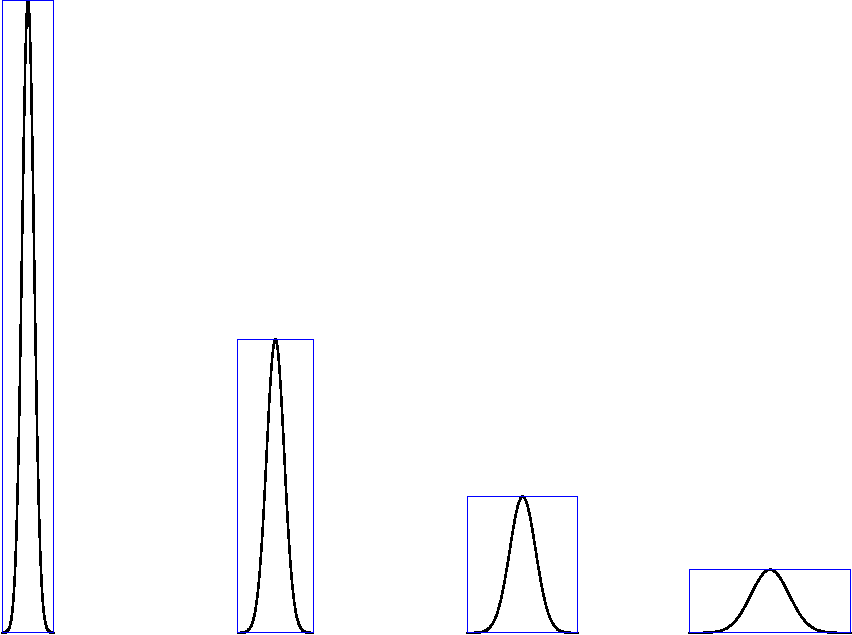
\includegraphics[width=2.5in]{heatscaling}
\quad
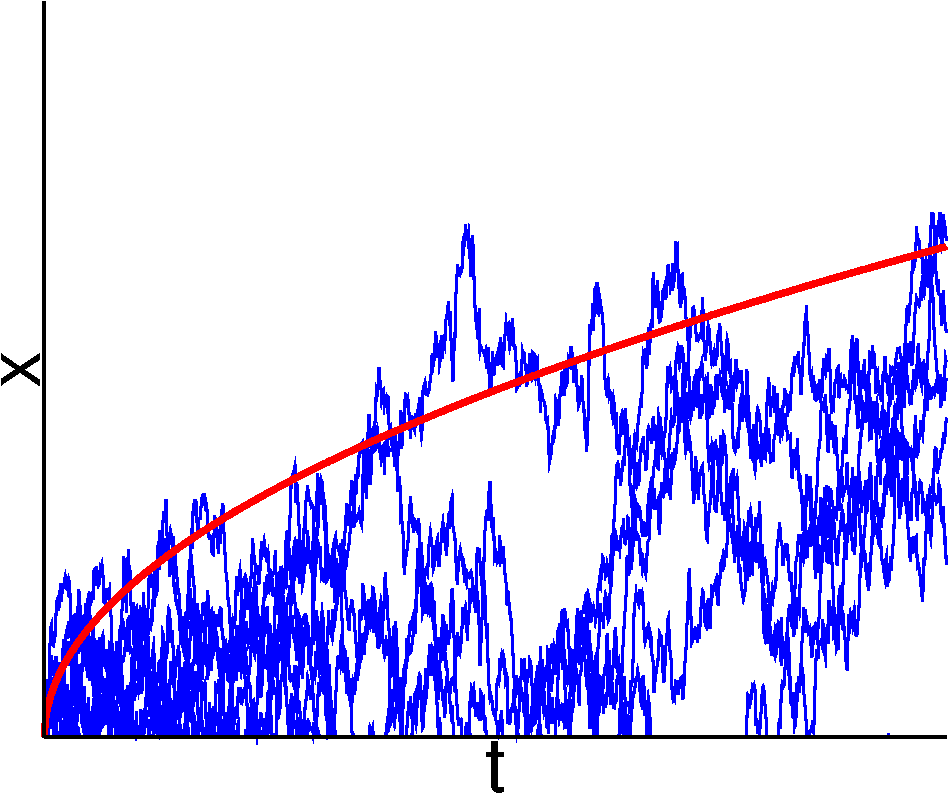
\includegraphics[width=2.5in]{brownian}

\emph{increasing time} $\to$ \qquad FIXME: parbox {\emph{historical note}:  in 1905 Einstein saw that the average distance traveled by particles in thermal motion scales like $\sqrt{t}$, so $s = t^{-1/2}x$ is an invariant}
\end{center}

similarity solutions

\begin{itemize}
\item Green's function of heat equation in 1D is
	$$u(t,x) = C\, t^{-1/2} e^{-x^2/(4Dt)}$$
\item ``similarity'' variables for 1D heat equation are
	$$s \stackrel{\text{\emph{input scaling}}}{\phantom{\Big|}=\phantom{\Big|}} t^{-1/2} x, \qquad u(t,x) \stackrel{\text{\emph{output scaling}}}{\phantom{\Big|}=\phantom{\Big|}} t^{-1/2} \phi(s)$$
\end{itemize}

\subsubsection*{An exact ``similarity'' solution to the SIA}

\begin{itemize}
\item jump forward to 1981
\item P.~Halfar found the similarity solution of the SIA in the case of flat bed and no surface mass balance \nocite{Halfar81,Halfar83}
\item Halfar's 2D solution for Glen flow law with $n=3$ has scalings
   $$H(t,r)=t^{-1/9} \phi(s), \qquad s = t^{-1/18} r$$
\item \dots so the diffusion of ice really slows down as the shape flattens out!
\end{itemize}

Halfar solution to the SIA: the movie

%\animategraphics[autoplay,loop,height=7.0cm]{4}{anim/halfar}{0}{26}

frames from $t=4$ months to $t = 10^6$ years, equal spaced in \emph{exponential} time

Halfar solution to the SIA: the formula

\begin{itemize}
\item for $n=3$ the solution formula is:
  $$H(t,r) = H_0 \left(\frac{t_0}{t}\right)^{1/9} \left[1 - \left(\left(\frac{t_0}{t}\right)^{1/18} \frac{r}{R_0}\right)^{4/3}\right]^{3/7}$$
\item the ``characteristic time'' is
  $$t_0 = \frac{1}{18 \Gamma} \left(\frac{7}{4}\right)^3 \frac{R_0^4}{H_0^{7}}$$
if $H_0$, $R_0$ are central height and ice cap radius at $t=t_0$
\item you choose $H_0$ and $R_0$ and then determine $t_0$
\item it is a simple formula to use for verification!
\end{itemize}

is the Halfar solution \emph{good for any modeling}?

\begin{itemize}
\item John Nye and others (2000)\nocite{NyeIcarus2000} compared the long-time consequences of different flow laws for the South Mars Polar Cap
\item they evaluated $\text{CO}_2$ ice and $\text{H}_2\text{O}$ ice softness parameters
\item \dots by comparing the long-time behavior of the corresponding Halfar solutions
\item conclusions:
  \begin{quote}
  \dots none of the three possible [$\text{CO}_2$] flow laws will allow a 3000-m cap, the thickness suggested by stereogrammetry, to survive for $10^7$ years, indicating that the south polar ice cap is probably not composed of pure $\text{CO}_2$ ice \dots the south polar cap probably consists of water ice, with an unknown admixture of dust.
  \end{quote}
\end{itemize}

\subsubsection*{Verifying the SIA scheme}

\begin{itemize}
\item where to get exact solutions for ice flow models?
  \begin{itemize}
  \item[$\circ$] textbook: Greve and Blatter (2009)\nocite{GreveBlatter2009}
  \item[$\circ$] similarity solutions to SIA (Halfar 1983\nocite{Halfar83}; Bueler et al 2005\nocite{BLKCB})
  \item[$\circ$] manufactured solutions to thermo-coupled SIA (Bueler et al 2007\nocite{BBL})
  \item[$\circ$] flowline and cross-flow SSA solutions (van der Veen, 1985; Schoof, 2006)\nocite{SchoofStream,vanderVeen85}
  \item[$\circ$] flowline Blatter solutions (Glowinski and Rappaz 2003)\nocite{GlowinskiRappaz}
  \item[$\circ$] flowline Stokes solutions for constant viscosity (Ladyzhenskaya 1963\nocite{Ladyzhenskaya}, Balise and Raymond 1985\nocite{BaliseRaymond1985})
  \item[$\circ$] manufactured solutions to the Stokes equations (Sargent and Fastook 2010; Jouvet and Rappaz 2011)\nocite{JouvetRappaz2011,SargentFastook2010}
  \end{itemize}
\end{itemize}

verifying SIA code vs Halfar

\begin{verbatim}
octave:40> verifysia(20)
average abs error            = 22.310
maximum abs error            = 227.849
octave:41> verifysia(40)
average abs error            = 9.490
maximum abs error            = 241.470
octave:42> verifysia(80)
average abs error            = 2.800
maximum abs error            = 155.796
octave:43> verifysia(160)
average abs error            = 1.059
maximum abs error            = 109.466
\end{verbatim}


\subsection{Applying our numerical ice sheet model}

demonstrate robustness

see \texttt{roughice.m}, which calls \texttt{siaflat.m} after setting-up the nasty initial state at left:

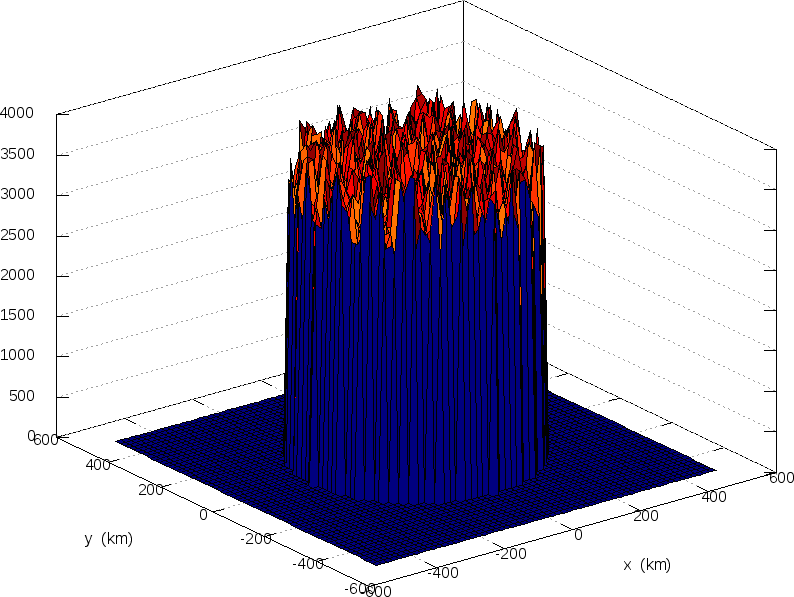
\includegraphics[width=2.5in]{roughinitial}
\quad
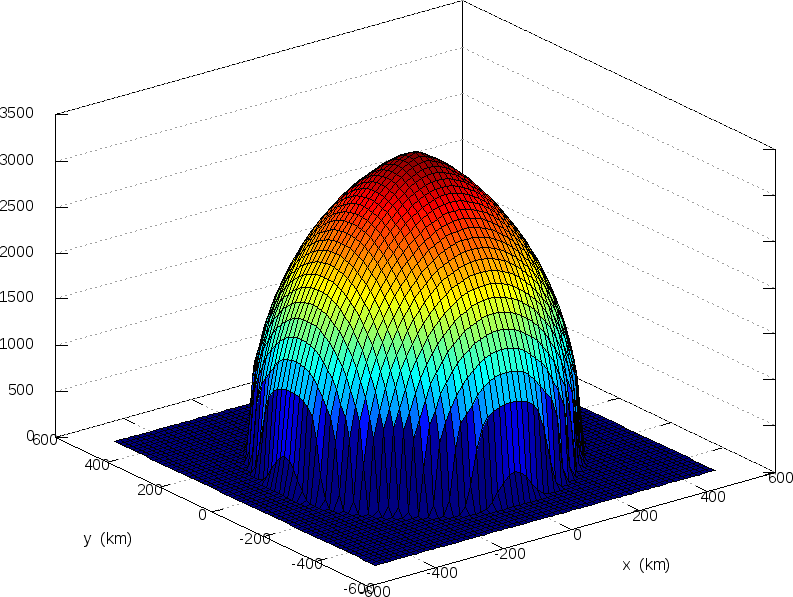
\includegraphics[width=2.5in]{roughfinal}

model the Antarctic ice sheet

\begin{itemize}
\item with careful-but-small modifications of \texttt{siaflat.m}, which make a good exercise:
  \begin{itemize}
  \item[$\circ$] observed accumulation as surface mass balance,
  \item[$\circ$] allow non-flat bed (so $H\ne h$),
  \item[$\circ$] differentiate the surface correctly where floating, and
  \item[$\circ$] calve at current calving front location
  \end{itemize}
here are results from this \emph{toy} Antarctic flow model
\item a 2000 model year run on a $\Delta x=50$ km grid; runtime a few seconds
\end{itemize}

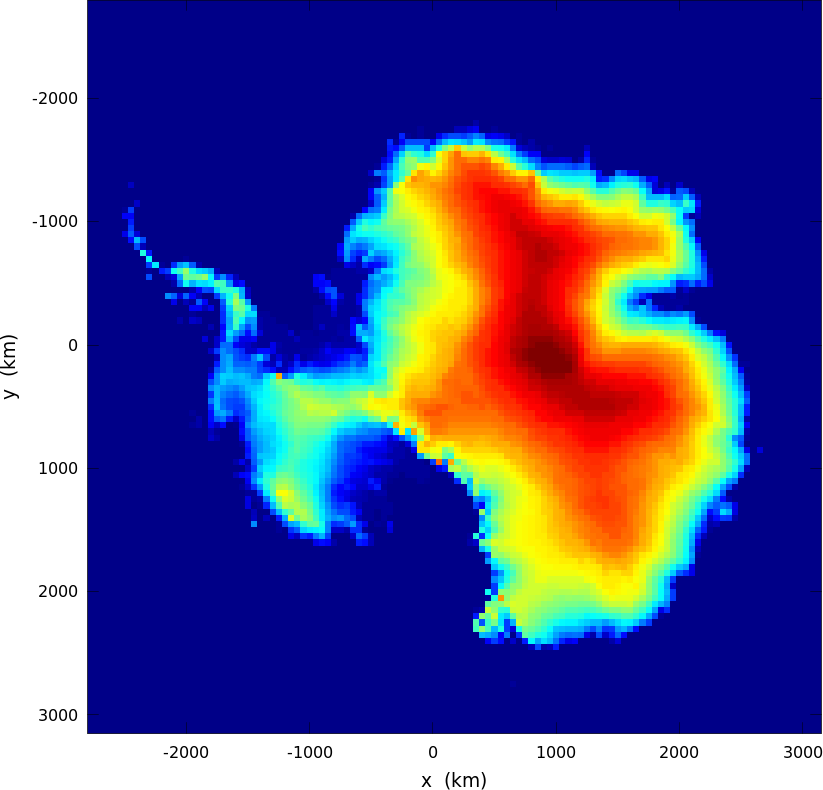
\includegraphics[width=2.5in]{antinitial}
\quad
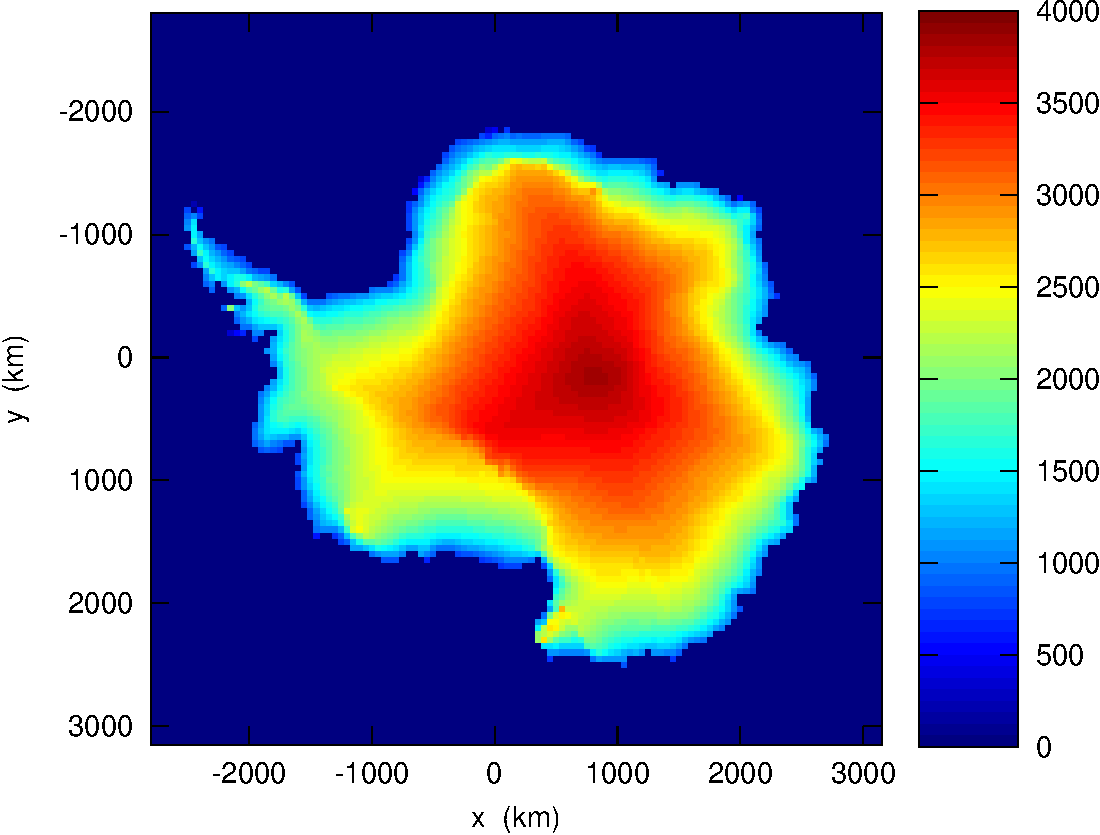
\includegraphics[width=2.5in]{antfinal}



\subsection{Mass continuity and kinematical equations}

the most basic shallow assumption:

\begin{itemize}
\item there are many shallow theories: SIA, SSA, hybrids, Blatter, \dots \nocite{Blatter}
\item \emph{all} make one assumption not required in the (non-shallow) Stokes theory:

\begin{center}
\emph{the surface and base of the ice are given by differentiable functions} $z=h(t,x,y)$ \emph{and} $z=b(t,x,y)$
\end{center}
\item surface overhang is not allowed
\end{itemize}


\begin{center}
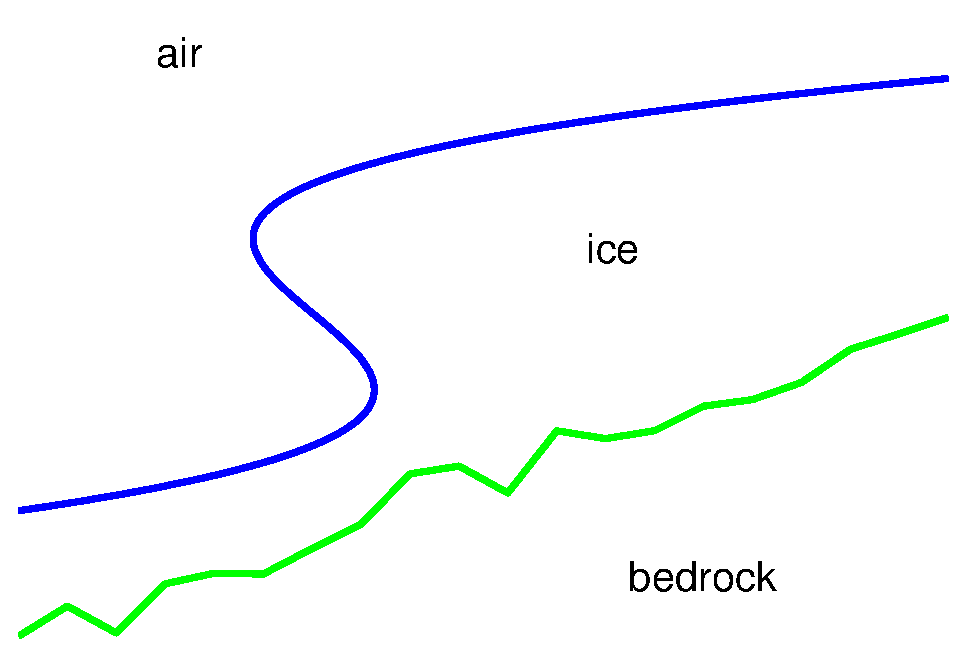
\includegraphics[width=2.5in]{sshape}
\quad
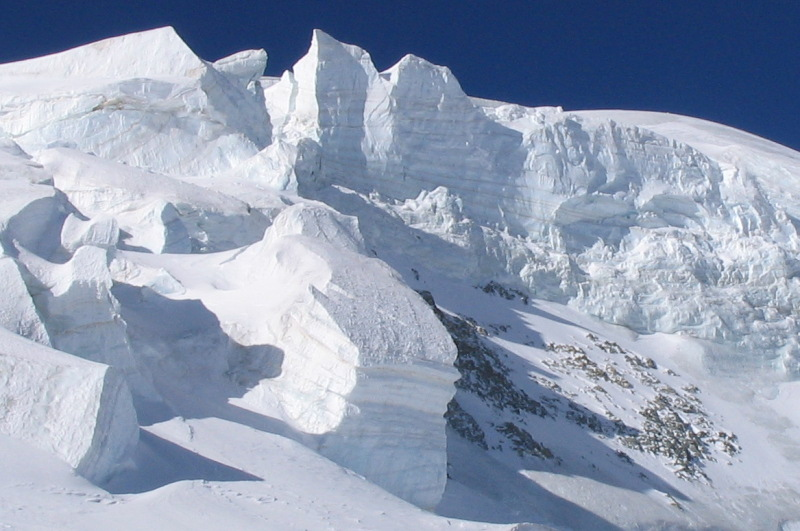
\includegraphics[width=2.5in]{Serac2}

\alert{not shallow!}
\end{center}


kinematic and mass continuity equations:

\begin{itemize}
\item what does this ``most basic shallow assumption'' get you?
\item \emph{answer:} a map-plane mass continuity equation
\item consider these three equations (\emph{on next slide}):
  \begin{itemize}
  \item[$\circ$]  the surface kinematical equation
  \item[$\circ$]  the base kinematical equation
  \item[$\circ$]  the map-plane mass continuity equation
  \end{itemize}
\item under the ``most basic shallow assumption'', 

\begin{center}\emph{any two imply the third}\end{center}
\item you connect the three equations by
  \begin{itemize}
  \item[$\circ$]  the incompressibility of ice
    $$u_x + v_y + w_z = 0$$
  \item[$\circ$]  and the Leibniz rule for differentiating integrals
  \scriptsize
    $$\frac{d}{dx}\left(\int_{g(x)}^{f(x)} h(x,y)\,dy\right) = f'(x) h(x,f(x)) - g'(x) h(x,g(x)) + \int_{g(x)}^{f(x)} h_x(x,y)\,dy$$
  \end{itemize}
\end{itemize}

\begin{itemize}
\item let $a$ be the surface mass balance function ($a>0$ is accumulation), and
\item $s$ be the basal melt rate function ($s>0$ is basal melting), so
\item $M=a-s$
\item define the map-plane flux of ice,
	$$\bq = \int_{b}^{h} (u,v)\,dz = \overline{\mathbf{u}}\,H$$
\item the three equations are:
\begin{empheq}[left=\text{surface kinematical}\quad,innerbox=\fbox]{equation}
h_t = a - u\big|_h h_x - v\big|_h h_y + w\big|_h  \label{surfkine}
\end{empheq}
\begin{empheq}[left=\text{base kinematical}\quad,innerbox=\fbox]{equation}
b_t = s - u\big|_b b_x - v\big|_b b_y + w\big|_b  \label{basekine}
\end{empheq}
\begin{empheq}[left=\text{mass continuity}\qquad\qquad\quad,innerbox=\fbox]{equation}
H_t = M - \Div \bq \label{masscontinuity}
\end{empheq}
\end{itemize}

\begin{itemize}
\item literature is full of incomplete calculations of these shallow equivalences
\item \dots usually mixed in with small-parameter arguments about shallow stress balances
\item most ice sheet models use the mass continuity equation to describe change in ice sheet geometry
\item \dots but they could instead use the surface kinematical equation
\end{itemize}

standard recipe for ice sheet models:

\begin{itemize}
\item the ingredients of a typical ice sheet model:
  \begin{enumerate}
  \item numerical implementation of a stress balance: gives velocity $(u,v,w)$
  \item from the horizontal velocity $(u,v)$ and the surface balance, do time-step of mass continuity equation to get $H_t$
  \item update upper and lower surface elevation
  \item decide on time-step, and repeat at 1.
  \end{enumerate}
\end{itemize}



\subsection{Shelves and streams}


\subsubsection*{shallow shelf approximation (SSA)}

flow model II: shallow shelf approximation (SSA) stress balance:
  
SSA model applies very well to \alert{ice shelves}:
\begin{itemize}
\item \dots for parts away from grounding lines
\item \dots and away from calving fronts
\end{itemize}

\begin{center}
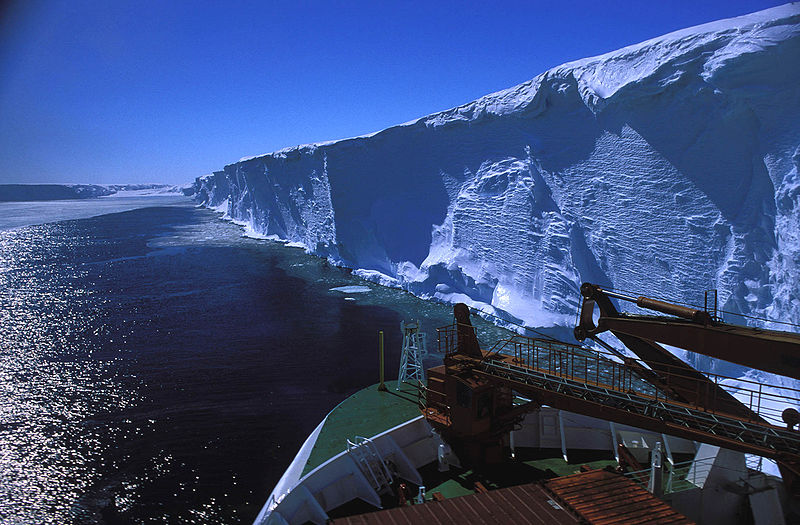
\includegraphics[width=2.5in]{ice_shelf_edge_hg}
\quad
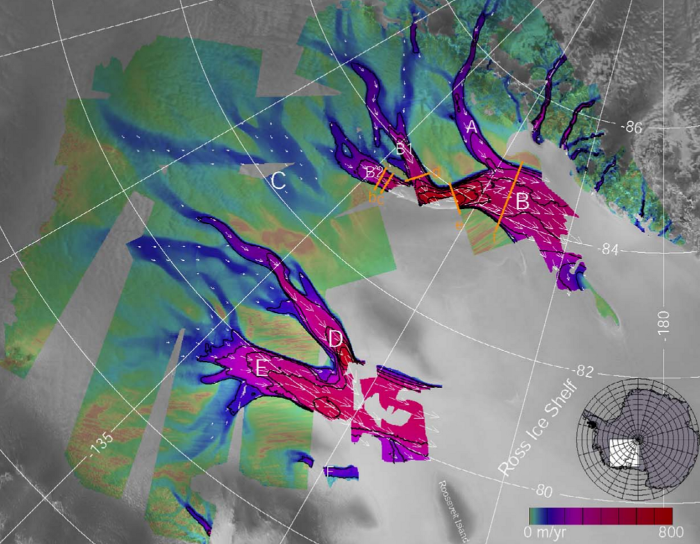
\includegraphics[width=2.5in]{siple}

edge of Ekstr\"om ice shelf (photo Hans Grobe) \qquad RADARSAT-derived surface velocity for Siple Coast ice streams, Antarctica
\end{center}

SSA also applies reasonably well to \alert{ice streams}:
\begin{itemize}
\item \dots with modest bed topography
\item \dots and weak bed strength\footnote{energy conservation (= ice temperature and basal melt) is a major aspect of ice stream flow \cite{Raymondenergy}, but not addressed here}
\item imperfect near shear margins and grounding lines
\end{itemize}


what is, \emph{and is not}, an ice stream?:

\begin{itemize}
\item ice streams 
  \begin{itemize}
  \item[$\circ$] slide ($100$ to $1000 \,\text{m}\,\text{a}^{-1}$)
  \item[$\circ$] concentration of vertical shear in a thin layer near base
  \item[$\circ$] \emph{liquid water} at bed plays a critical role (Clarke, 2005)\nocite{Clarke05}
  \end{itemize}
\item ``outlet glaciers''
  \begin{itemize}
  \item[$\circ$] fast surface speed (up to $10 \,\text{km}\,\text{a}^{-1}$)
  \item[$\circ$] uncertain how much is sliding
  \item[$\circ$] substantial vertical shear ``up'' in the ice column,
  \item[$\circ$] not-at-all flat bed topography
  \item[$\circ$] soft, temperate ice may play a big role
  \end{itemize} 
\item \alert{few simplifying assumptions are appropriate for outlet glaciers}
\end{itemize}

\begin{center}
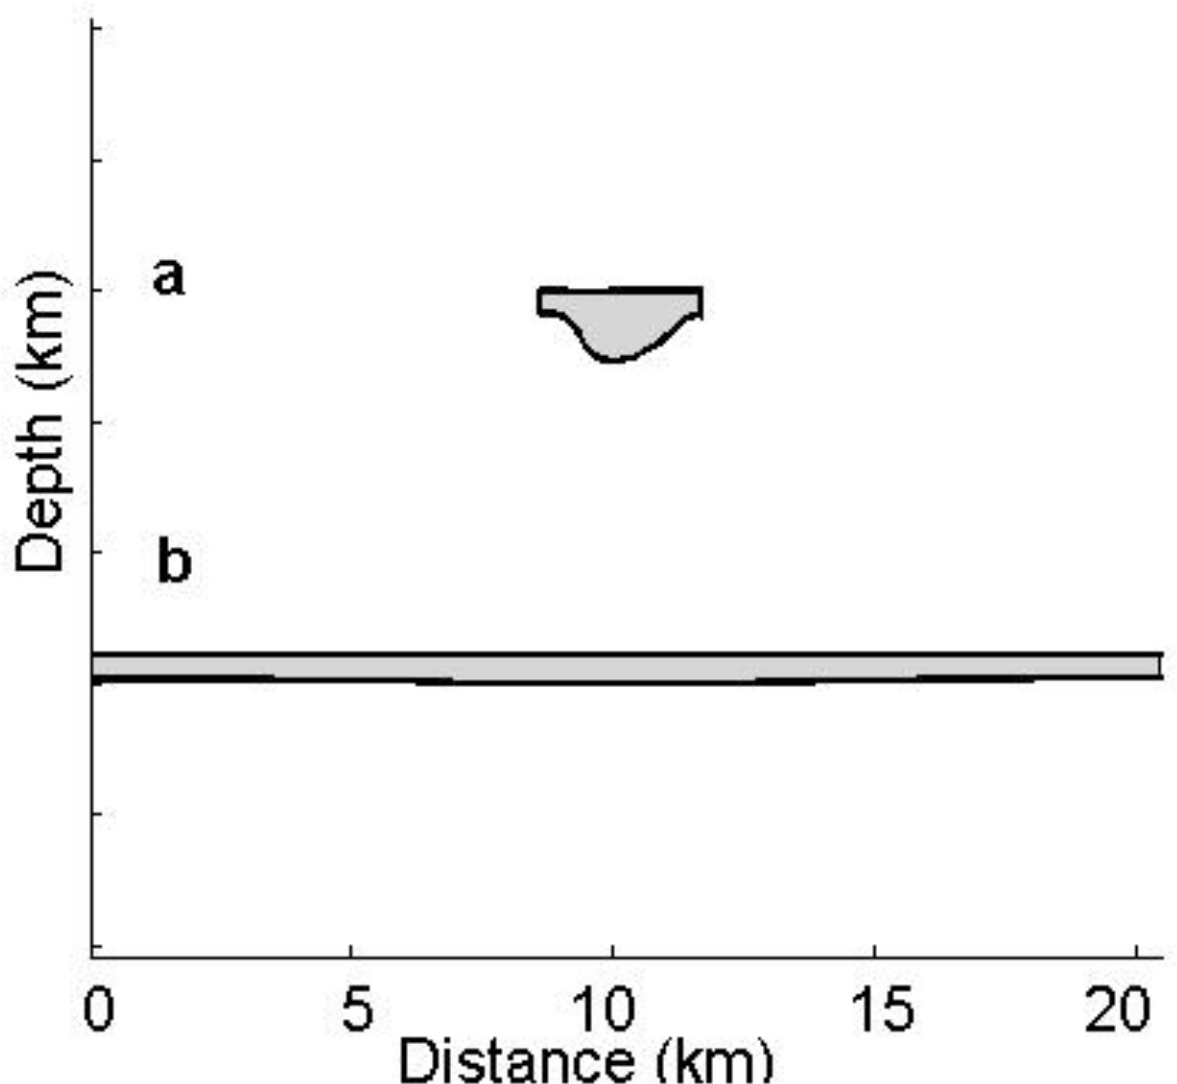
\includegraphics[width=3.0in]{streamisbrae}

Cross sections of Jakobshavns Isbrae (\textbf{a}) and Whillans Ice Stream (\textbf{b}).  Plotted without vertical exaggeration.  (Figure 1 in \cite{TrufferEchelmeyer})
\end{center}

SSA stress balance equation:

\begin{itemize}
\item only plane flow case (``flow line'')
\item the stress balance equation which determines velocity in an \emph{ice stream}:
\begin{empheq}[box=\fbox]{equation}
  \left({\color{red}2 A^{-1/n} H |u_x|^{1/n - 1} u_x}\right)_x - {\color{blue}C|u|^{m-1}u} = {\color{green}\rho g H h_x} \label{ssa}
\end{empheq}
\item the {\color{red} red term} inside parentheses is the vertically-integrated ``longitudinal'' or ``membrane'' stress
\item the {\color{blue} blue term} is basal resistance
\item the {\color{green} green term} is  driving stress
\item derived originally by \cite{Morland,MacAyeal}
\item \emph{how to think about this equation}?
\item \emph{how do you solve it numerically}?
\end{itemize}

flow line model: from stream to shelf:
\begin{align*}
  u = u_0 & \qquad \text{ at } x = 0 \\
  \left.\begin{array}{r}
  \left(2 A^{-1/n} H |u_x|^{1/n - 1} u_x\right)_x - C|u|^{m-1}u = \rho g H h_x \\
  h = H + b
  \end{array}\right\}& \qquad \text{ on } 0 < x < x_g \\
  \left.\begin{array}{r}
  \left(2 A^{-1/n} H |u_x|^{1/n - 1} u_x\right)_x + 0 = \rho g H h_x \\
  h = (1-\rho/\rho_w) H
  \end{array}\right\}& \qquad \text{ on } x_g < x < x_c \\
  2 A^{-1/n} H |u_x|^{1/n - 1} u_x = \frac{1}{2}\rho (1-\rho/\rho_w) g H^2 & \qquad \text{ at } x = x_c
\end{align*}

\subsubsection*{flotation criterion and grounding lines}

\begin{itemize}
\item the inequality ``$\rho H < - \rho_w b$'' is the \alert{flotation criterion}
\item at the grounding line $x=x_g$ the above inequality switches
\item \dots and the driving stress switches form:
  \begin{itemize}
  \item[$\circ$] on the grounded side we know $\rho H > - \rho_w b$ so
  	$$\rho g H h_x = \rho g H (H_x + b_x)$$
  \item[$\circ$] on the floating side we know $\rho H < - \rho_w b$ so $h = (1-\rho/\rho_w) H$ and so
  	$$\rho g H h_x = \rho(1-\rho/\rho_w) g H H_x$$
  \end{itemize}
\item also: $H,u,u_x$ are all continuous at $x=x_g$
\item best numerical models for moving grounding lines still an open question (e.g.~MISMIP and all that)
\end{itemize}


\subsubsection*{ice shelf flow line solution}

exact velocity and thickness for steady ice shelf:
\begin{itemize}
\item limited goal here: describe a steady state, 1D ice shelf
\item there is this nice \alert{by-hand} result (next slide): the thickness and velocity in the ice shelf can be completely determined \cite{MacAyealBarcilon,vanderVeen83} in terms of the 
  \begin{enumerate}
  \item ice thickness $H_g$ at the grounding line and
  \item ice velocity $u_g$ at the grounding line
  \end{enumerate}
\item we will use this to
  \begin{itemize}
  \item[$\circ$] understand the SSA better
  \item[$\circ$] verify a numerical SSA code
  \end{itemize}
\end{itemize}

see \texttt{testshelf.m} 

\begin{center}
  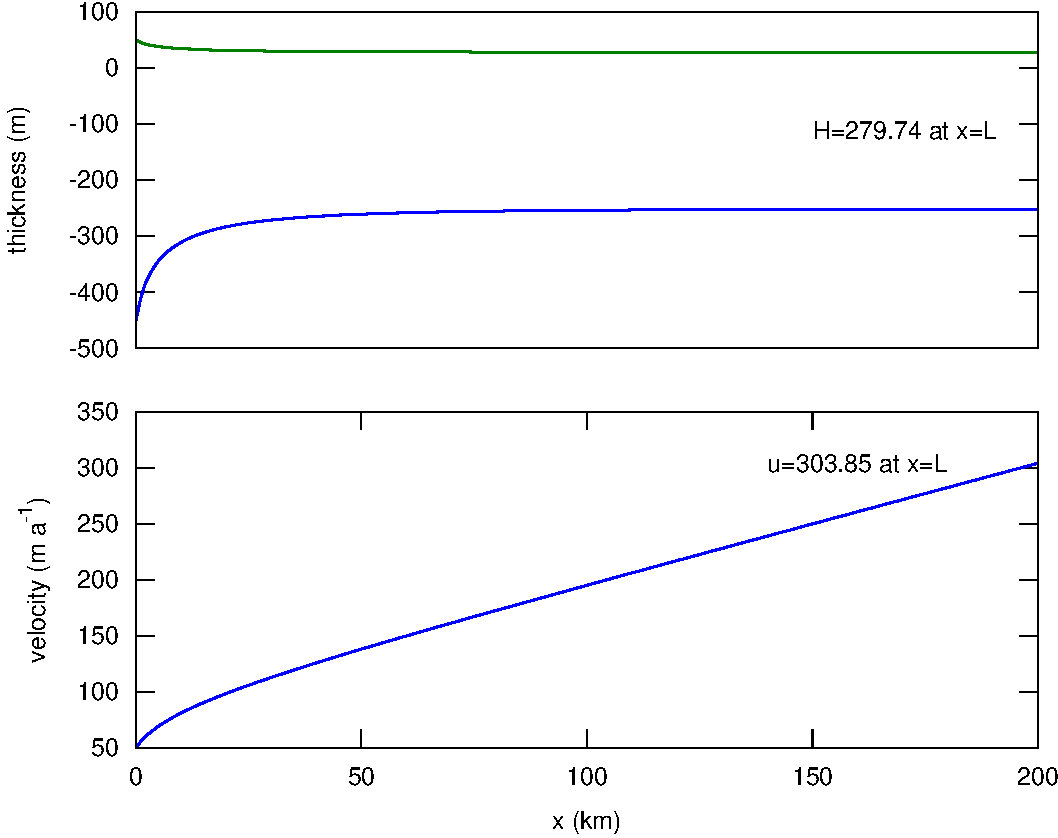
\includegraphics[width=3.0in]{steadyshelf} \hfill 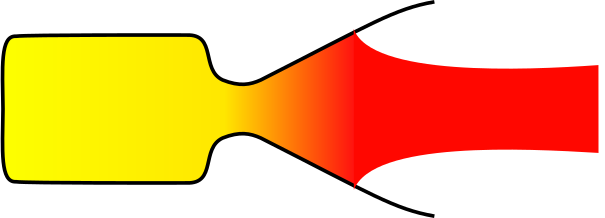
\includegraphics[width=2.5in]{Rocket_nozzle_expansion}
\end{center}


\subsubsection*{numerical SSA}

numerically solving the SSA stress balance:
\begin{itemize}
\item here we fix ice thickness $H(x)$ and find the velocity numerically
\item the stress balance is a nonlinear equation in the velocity:
  $$\left(2 A^{-1/n} H |u_x|^{1/n - 1} u_x\right)_x - C|u|^{m-1}u = \rho g H h_x$$
\item \alert{iteration is needed}
\item I'll describe the numerical method for a shelf \emph{or} stream, but only give a code for an ice shelf
\end{itemize}

\begin{itemize}
\item coefficient ${\color{red} \bar \nu} = A^{-1/n} |u_x|^{1/n-1}$ is the ``effective viscosity'':
   $$\left(2 \,{\color{red} \bar \nu}\, H u_x\right)_x - C |u|^{m-1} u = \rho g H h_x$$
\item \emph{simplest iteration idea}: use old effective viscosity to get new velocity solution, and repeat until things stop changing
  \begin{itemize}
  \item[$\circ$] this is ``Picard'' iteration
  \item[$\circ$] Newton iteration is a superior alternative
  \end{itemize}
\item specifically:
  \begin{itemize}
  \item[$\circ$] last iterate $u^{(k-1)}$
  \item[$\circ$] define $W^{(k-1)} = 2 \bar \nu H = 2 A^{-1/n} |u^{(k-1)}_x|^{1/n-1} H$
  \item[$\circ$] current iterate (unknown) $u^{(k)}$
  \item[$\circ$] solve repeatedly:
     $$\left(W^{(k-1)} u^{(k)}_x\right)_x - C |u^{(k-1)}|^{m-1} u^{(k)} = \rho g H h_x$$
  \end{itemize}
\end{itemize}

solving the ``inner'' linear problem:
\begin{itemize}
\item abstract the problem:
   $$\left(W(x)\, u_x\right)_x - \alpha(x)\, u = \beta(x)$$
on $0 < x < L$, with boundary conditions
   $$u(0) = V, \qquad  u_x(L) = \gamma$$
\item an \emph{elliptic} PDE boundary value problem
\item $W(x)$, $\alpha(x)$, $\beta(x)$ are known functions in the SSA context:
  \begin{itemize}
  \item[$\circ$] both $W(x)$ and $\alpha(x)$ come from previous iteration
  \item[$\circ$] $\beta(x)$ is driving stress
  \end{itemize}
\end{itemize}

where do you get an initial guess $u^{(0)}$?:

\begin{itemize}
\item \emph{for floating ice}, a possible initial guess for velocity comes from assuming a uniform strain rate:
   $$u^{(0)}(x) = \gamma (x-x_g) + u_g$$
where $\gamma$ is the value of $u_x$ found from calving front stress imbalance
\item \emph{for grounded ice}, a possible initial guess for velocity is to assume ice is held by basal resistance only:
   $$u^{(0)}(x) = \left(-C^{-1} \rho g H h_x\right)^{1/m}$$
\end{itemize}

numerics of the ``inner'' linear problem:

\begin{itemize}
\item suppose $j=1,2,\dots,J+1$, where $x_1 = x_g$ and $x_{J+1} = x_c$ are endpoints
\item $W(x)$ is needed on the staggered grid; the approximation is:
$$\frac{W_{j+1/2} (u_{j+1} - u_j) - W_{j-1/2} (u_{j} - u_{j-1})}{\Delta x^2} - \alpha_j u_j \stackrel{\ast}{=} \beta_j$$
\item left-hand boundary condition: $u_1 = V$ given
\item right-hand boundary condition (``$u_x(L)=\gamma$''):
  \begin{itemize}
  \item[$\circ$] introduce notional point $x_{J+2}$
  \item[$\circ$]
    $$\frac{u_{J+2} - u_J}{2 \Delta x} = \gamma$$
  \item[$\circ$] using equation $\ast$ in $j=J+1$ case, eliminate $u_{J+2}$ variable ``by-hand'' before coding numerics \nocite{MortonMayers}
  \end{itemize}
\end{itemize}

\begin{itemize}
\item so SSA stress balance has form  \quad $A \mathbf{x} = \mathbf{b}$, \quad namely:
$$
\begin{bmatrix}
1 &  &  &  &  \\
W_{3/2} & A_{22} & W_{5/2} &  &  \\
 & W_{5/2} & A_{33} &  &  \\
 &  & \ddots & \ddots &  \\
 &  & W_{J-1/2} & A_{JJ} & W_{J+1/2} \\
 &  &  & A_{J+1,J} & A_{J+1,J+1} \\
\end{bmatrix}\,
\begin{bmatrix}
u_1 \\ u_2 \\ u_3 \\ \vdots \\ u_J \\ u_{J+1}
\end{bmatrix}
=
\begin{bmatrix}
0 \\ \beta_2 \Delta x^2 \\ \beta_3 \Delta x^2 \\ \vdots \\ \beta_J \Delta x^2 \\ b_{J+1}
\end{bmatrix}
$$
\item with diagonal entries
$$A_{22} = -(W_{3/2}+W_{5/2}+\alpha_1 \Delta x^2)$$
$$A_{33} = -(W_{5/2}+W_{7/2}+\alpha_2 \Delta x^2)$$
and so on, up to $A_{JJ}$, 
\item with special cases in last equation:
$$A_{J+1,J} = 2 W_{J+1/2}$$
$$A_{J+1,J+1} = -(2 W_{J+1/2}+\alpha_{J+1}\Delta x^2)$$
$$b_{J+1} = -2 \gamma \Delta x W_{J+3/2} + \beta_{J+1} \Delta x^2$$
\item this is a \emph{tridiagonal} system
\end{itemize}

\minput{flowline}

\subsubsection*{Testing the parts}

testing the ``inner'' linear code

\begin{itemize}
\item before proceeding to solve nonlinear SSA problem, we can test the ``abstracted'' code \texttt{flowline.m}
\item test by ``manufacturing'' solutions
  \begin{itemize}
  \item[$\circ$] see \texttt{testflowline.m}; not shown
  \end{itemize}
\item results:
  \begin{itemize}
  \item[$\circ$] converges at optimal rate $O(\Delta x^2)$
  \end{itemize}
\end{itemize}


\minput{ssaflowline}

\emph{numerical} thickness and velocity for steady ice shelf:

lines below are a convergence analysis of \texttt{testshelf.m}, which calls \texttt{ssaflowline.m}:

\begin{center}
  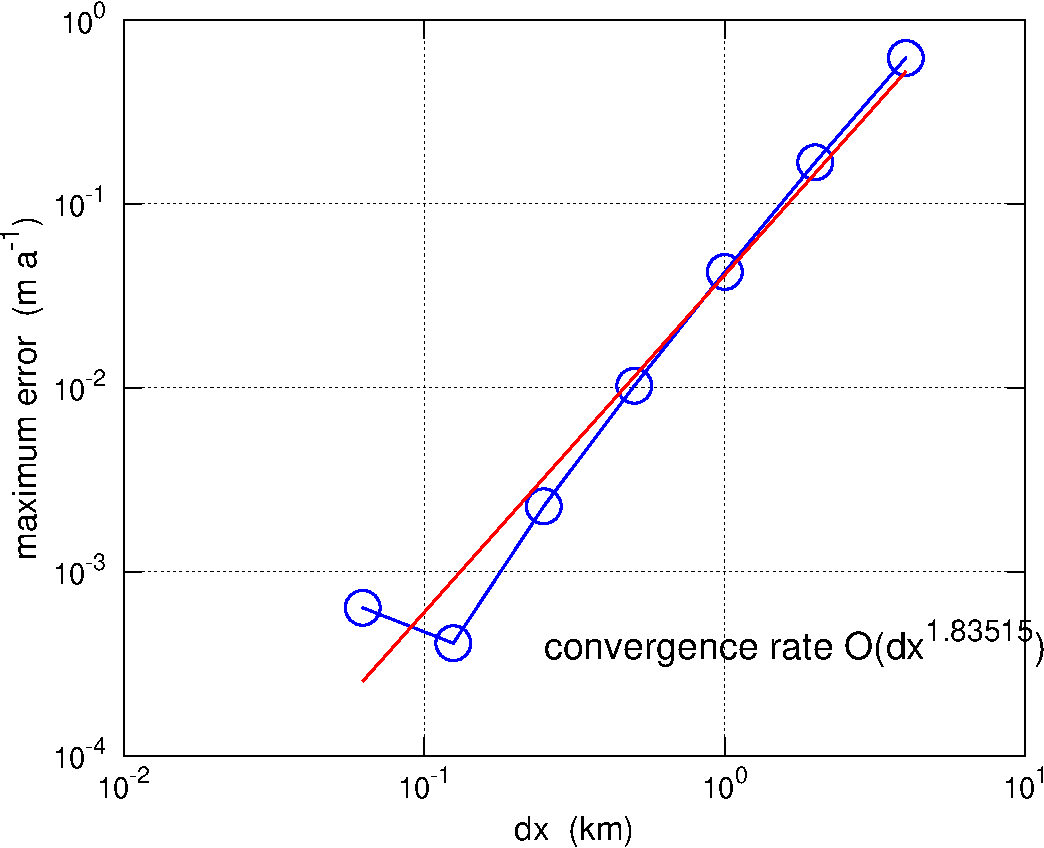
\includegraphics[width=3.0in]{shelfconv}
\end{center}

\subsubsection*{realistic ice shelf modeling}

\begin{itemize}
\item flow lines are never very realistic
\item you can add ``side drag'' \dots but I don't really know how to parameterize it
\item also, ice shelves have surprises:
  \begin{itemize}
  \item[$\circ$] high basal melt near grounding lines
  \item[$\circ$] marine ice can freeze-on at bottom (below)
  \item[$\circ$] ``reverse slope'' bed instability and WAIS \dots
  \end{itemize}
\end{itemize}

\medskip
\begin{center}
  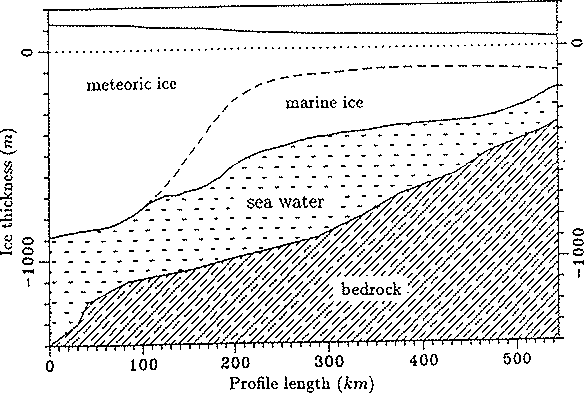
\includegraphics[width=3.0in]{marineice}
  
from Grosfeld \& Thyssen 1994 \nocite{GrosfeldThyssen1994}
\end{center}

ice shelf modeling in 2D:

\begin{itemize}
\item ``diagnostic'' (static geometry) ice shelf modeling in two horizontal variables has been quite successful
\item observed surface velocities should validate stress balance models
  \begin{itemize}
  \item[$\circ$] Ross ice shelf example below using PISM
  \item[$\circ$] \dots but many models can do this (MacAyeal et al 1996\nocite{MacAyealetal})
  \end{itemize}
\end{itemize}

\begin{center}
  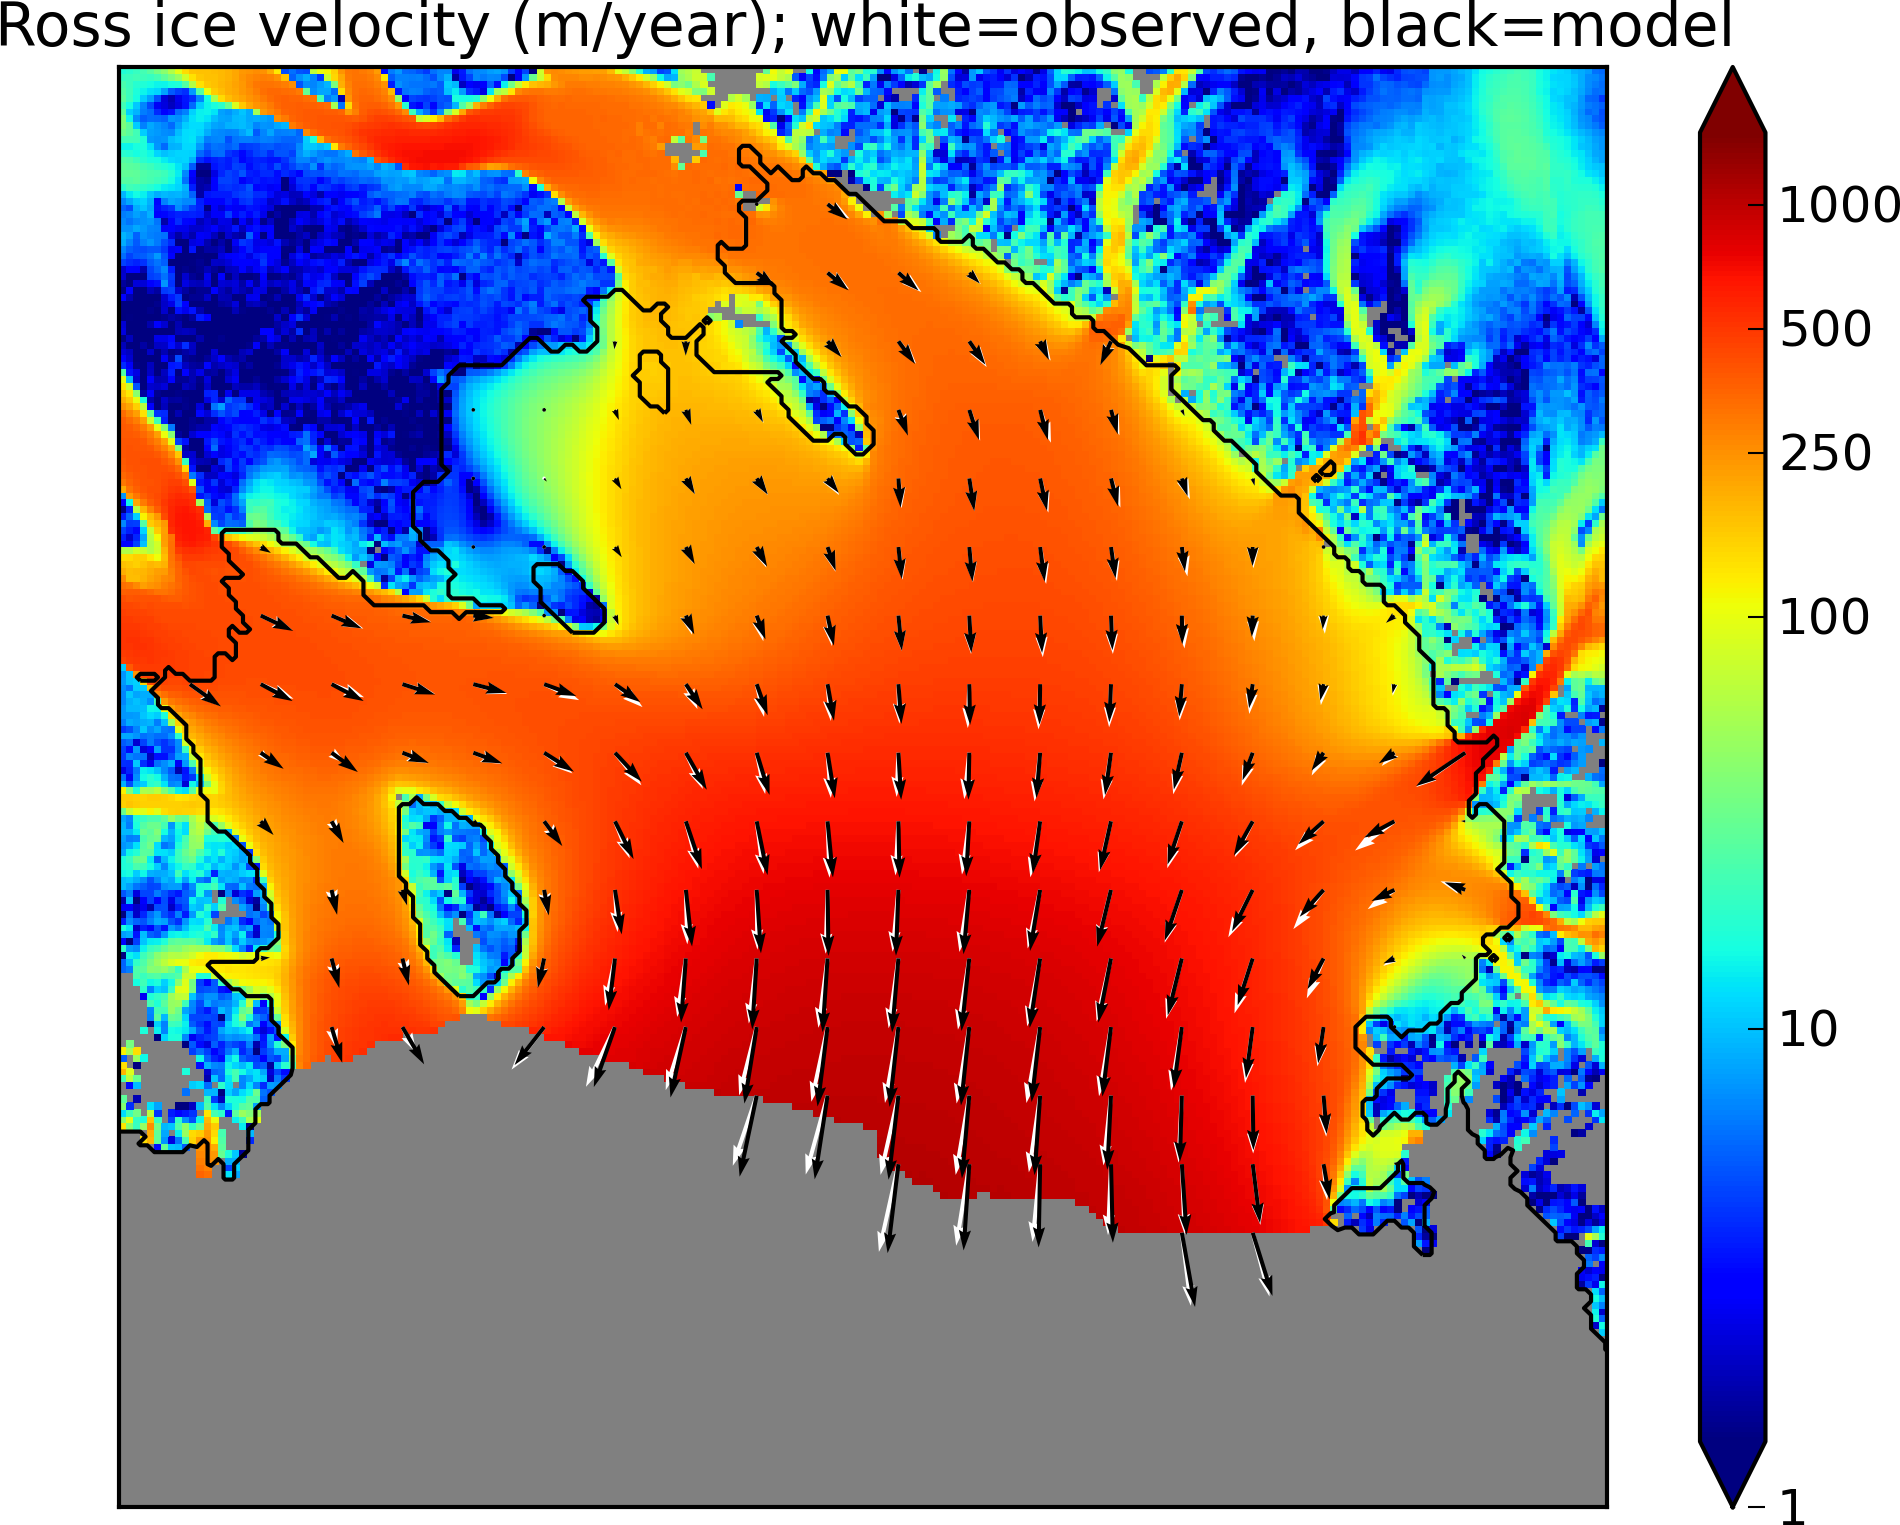
\includegraphics[width=2.5in]{rossquiver}
  \quad
  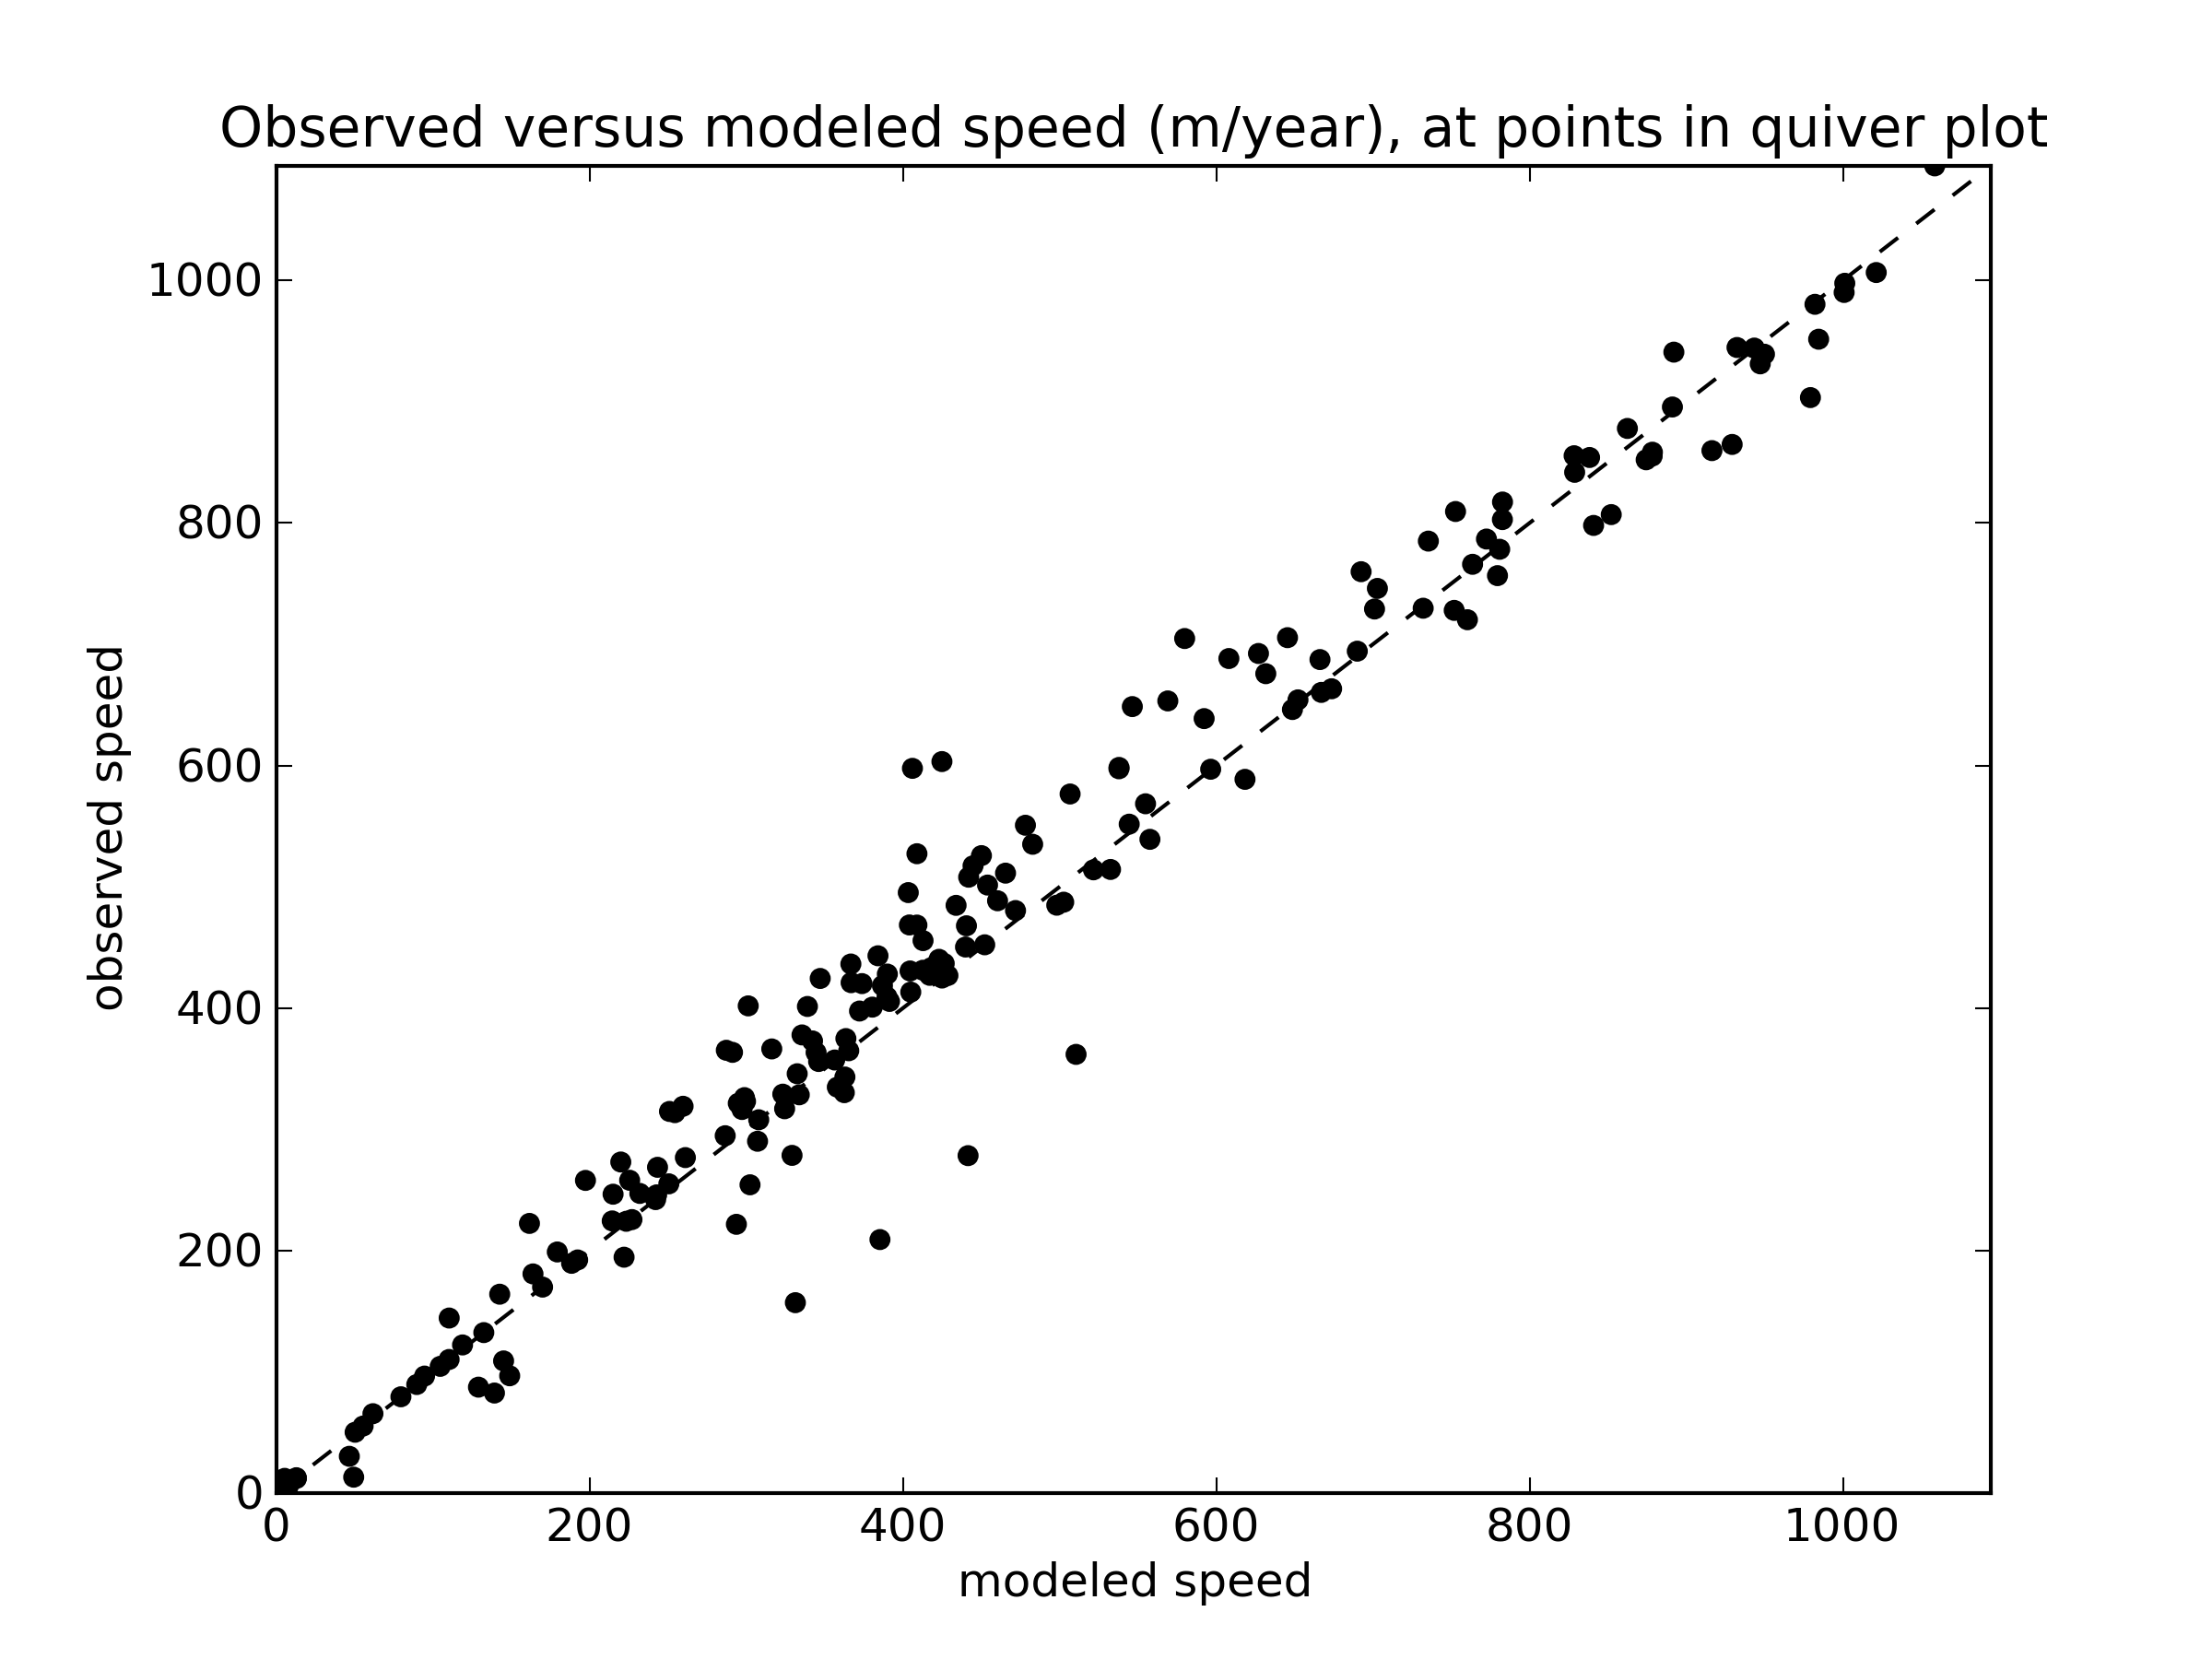
\includegraphics[width=2.5in]{rossscatter}
\end{center}


\subsection{A summary of numerical solutions}

\subsubsection*{numerical solution of stress balances: a summary}

\begin{itemize}
\item stress balance equations (e.g.~SSA) determine horizontal velocity from geometry and boundary conditions
  \begin{itemize}
  \item[$\circ$] nonlinear so iteration is necessary
  \item[$\circ$] at each iteration a sparse matrix ``inner'' problem is solved
  \item[$\circ$] give the ``inner'' problem to a matrix solver software package
  \end{itemize}
\item general principles: \emph{modularize your code} and \emph{test the parts}
\end{itemize}

\subsubsection*{numerical solution of the mass continuity equation: a summary}

\begin{itemize}
\item the \emph{mass continuity equation} is
  $$H_t = M - \nabla \cdot (\mathbf{u} H)$$
\item the numerical nature of this equation depends on the stress balance:
  \begin{itemize}
  \item[$\circ$] the equation is a diffusion for frozen bed, large scale flows (i.e.~SIA)
  \item[$\circ$] it is \emph{not} very diffusive for membrane stresses and no basal resistance (e.g.~SSA for ice shelves)
  \item[$\circ$] it is significantly diffusive for ice streams (but how much?)
  \item[$\circ$] there is not much helpful theory on to solve this transport problem
  \item[$\circ$] maybe \emph{you} will help find this theory!
  \end{itemize}
\end{itemize}


\subsection{Next steps}

\subsubsection*{practicalities}

technical skills for numerical ice sheet modeling:

\begin{itemize}
\item comfort in a technical computing environment; need to know:
  \begin{itemize}\small
  \item[$\circ$] an editor,
  \item[$\circ$] a scripting/prototyping language (Matlab, Python, etc.),
  \item[$\circ$] a compiled language (C or Fortran),
  \item[$\circ$] \emph{a version control system} (Subversion, git, etc.), and
  \item[$\circ$] some tools for NetCDF files
  \normalsize
  \end{itemize}
\item willingness to read math, numerical analysis, computer science, etc.
\item \emph{physics}
\item \emph{never} re-invent the wheel for basic numerics like these:
  \begin{itemize}
  \item[$\circ$] numerical linear algebra
  \item[$\circ$] mesh generation, finite element assembly and solve
  \item[$\circ$] \dots \emph{except} to write throw-away codes to help you understand numerical ideas 
  \end{itemize}
\item try existing ice flow models:
  \begin{itemize}
  \item[$\circ$] open source SIA-based comprehensive models: GLIMMER, SICOPOLIS
  \item[$\circ$] open source hybrid/higher-order/Stokes models: PISM, Elmer, ISSM
  \end{itemize}
\item ice sheet modeling is young, and much to do!
\end{itemize}


\subsubsection*{some omitted models}

thermomechanical coupling:

\begin{itemize}
\item ice softness $A(T)$ varies by $10^3$ in relevant temperature range
\end{itemize}

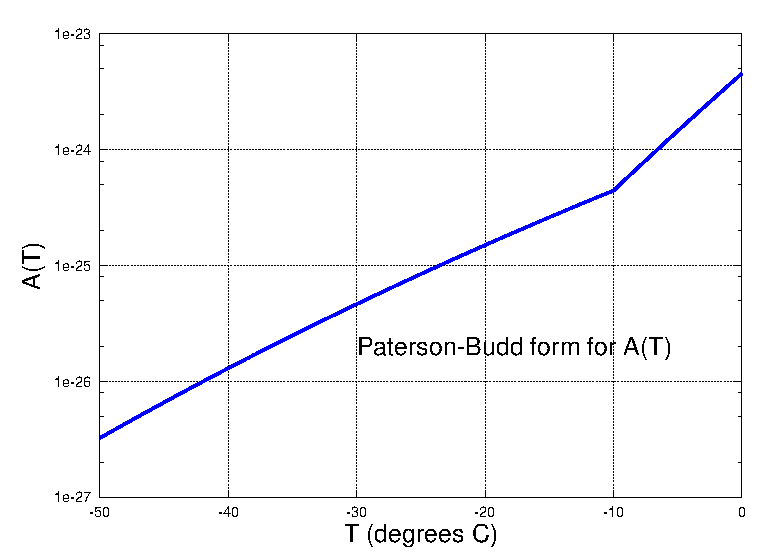
\includegraphics[width=3.0in]{AofT}


\begin{itemize}
\item ice thermal state (temperature) gives ice sheet flows their ``long memory'' of past climate
\item dissipation of gravitational potential energy is major part of basal melt
  \begin{itemize}
  \item[$\circ$] each year, Jakobshavn drainage basin in Greenland dissipates enough gravitational potential energy to melt $> 1\,\text{km}^3$ of ice
  \item[$\circ$] geothermal flux also significant in slow parts
  \end{itemize}
\item so good ice sheet models need conservation of energy
  \begin{itemize}
  \item[$\circ$] ``enthalpy'' is good way to track energy content polythermally (Aschwanden et al.~2012)\nocite{AschwandenBuelerKhroulevBlatter}
  \end{itemize}
\end{itemize}

solid Earth deformation:

\begin{itemize}
\item ice density is about $\frac{1}{3}$ that of rock in the Earth's mantle,
  \begin{itemize}
  \item[$\circ$] 1000 m of ice depresses the Earth's crust about 300 m
  \item[$\circ$] \dots if allowed enough time
  \item[$\circ$] how much time is determined by \emph{upper mantle viscosity}
  \item[$\circ$] \dots which is not perfectly known
  \end{itemize}
\item Earth deformation changes bed topography and thus ice flow
\item modeling Earth deformation is most important to modeling ice flow over long time scales (Peltier, 1998)\nocite{Peltier1998review}
\end{itemize}

\begin{center}
  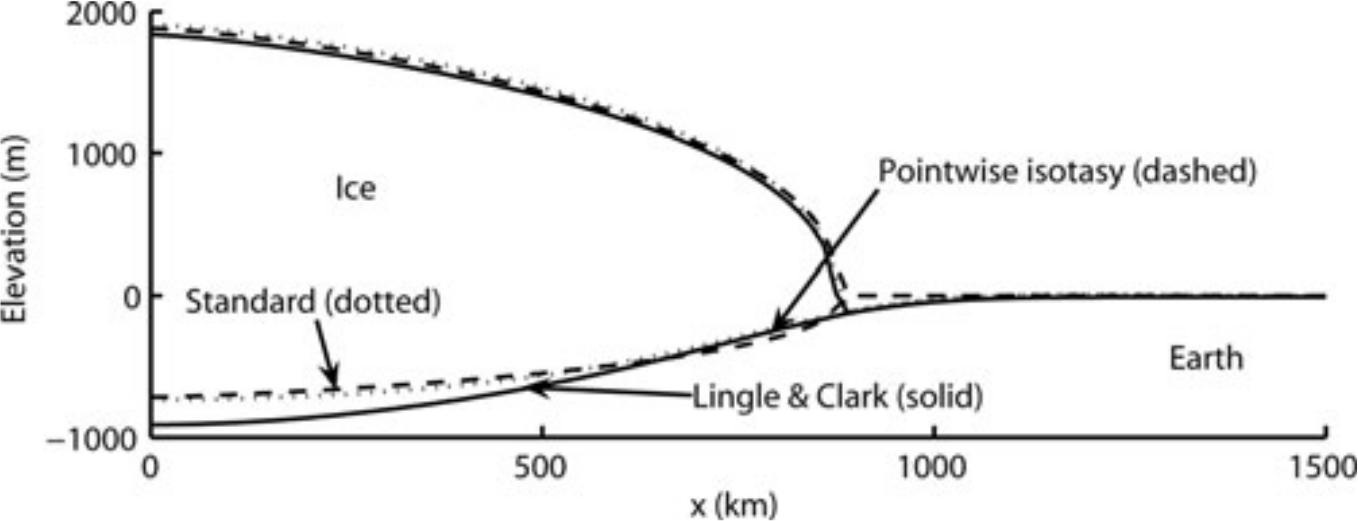
\includegraphics[width=3.0in]{earthcompare}
\end{center}

spin-up:

\begin{itemize}
\item direct observations are not enough to initialize an ice sheet flow model
  \begin{itemize}
  \item[$\circ$] because ice temperature is a ``hidden variable'', and
  \item[$\circ$] because sliding depends on additional liquid water ``hidden variables'' at base
  \end{itemize}
\item two options exist to initialize:
  \small
  \begin{enumerate}
  \item \emph{traditional choice}: use low-dimensional time series data from physical surrogates (e.g. $\delta \phantom{|}^{18}O$ record from ice cores) for paleoclimate record; hope a long model run ends with a good current state
  \item \emph{promising alternative}:  use rich and spatially-distributed mostly-surface observations of present ice sheet state to reconstruct initial state using ``inversion'' of PDEs
  \normalsize
  \end{enumerate}
\end{itemize}

inverse modeling:

\begin{itemize}
\item stress balance PDEs can turn extra boundary data on top into missing basal information
\item surface velocity observations can be inverted to find basal shear stress (below)
\item mostly future: invert radar layers (isochrones)
\end{itemize}

\begin{center}
  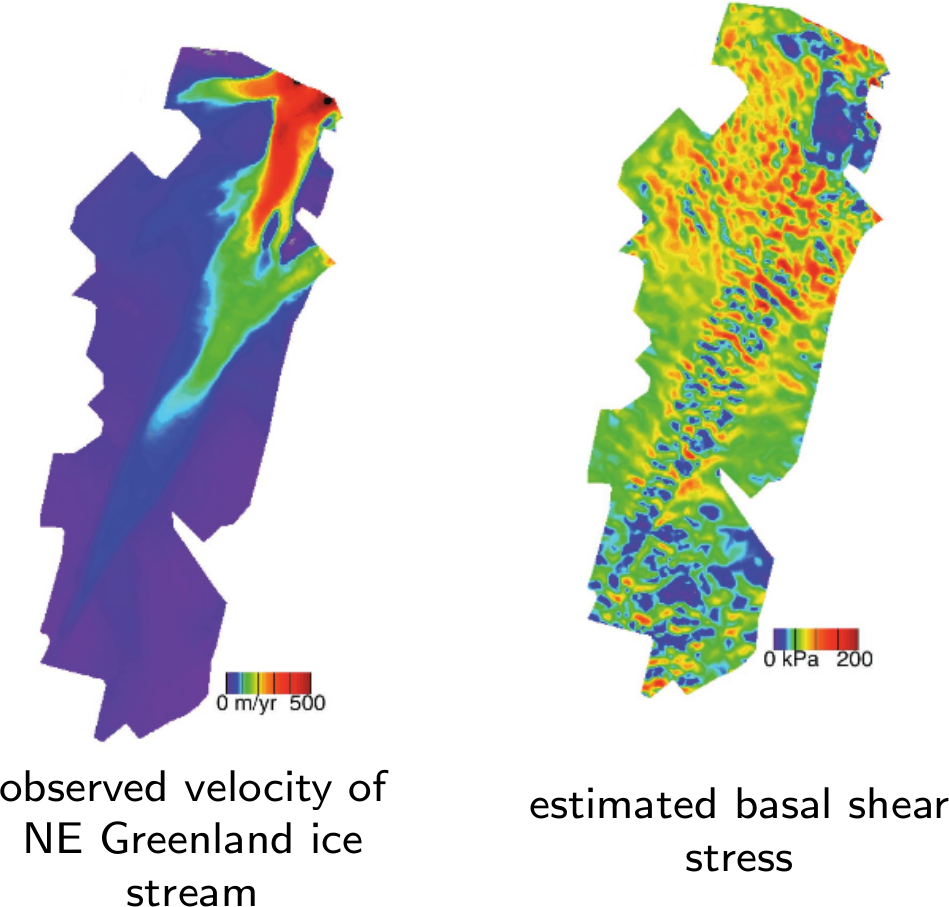
\includegraphics[width=3.0in]{NEgreenlandJoughin}
  
from Joughin et al.~(2001)\nocite{Joughinetal2001}
\end{center}

Stokes equations and solvers:

\begin{itemize}
\item the Stokes model itself, without shallow assumptions, can be solved numerically, \alert{but}:
  \begin{itemize}
  \item[$\circ$] many equations in many unknowns, especially in 3D
  \item[$\circ$] requires explicit accounting for incompressibility---a constraint on the flow---through a pressure variable
  \item[$\circ$] ice sheets are \emph{actually} shallow, and the aspect ratio of grid elements can be a problem
  \end{itemize}
\item much of the success so far is at a smaller scale
\end{itemize}



\subsection{Notes and references}

Not covered here:
  \begin{itemize}
  \item Stokes and ``higher order'' flow equations
  \item thermomechanical coupling or polythermal ice
  \item subglacial hydrology/processes
  \item mass balance and snow/firn processes
  \item constitutive relations other than Glen isotropic
  \item grounding lines, calving fronts, ocean interaction
  \item paleo-climate and ``spin-up''
  \item earth deformation under ice sheet load
  \item other numerics: FEM, spectral, multigrid, parallel, \dots
  \item etc.
  \end{itemize}

Where does the SIA come from?    Historically, it was derived several authors in the 1970s and 80s \cite{FowlerLarson1978,MorlandJohnson,Hutter} and thus it is recent compared to the Stokes model.  Logically, you scale the Stokes equations using smallness of $\eps = [H]/[L]$, where $[H]$ is a typical thickness of an ice sheet and $[L]$ is a typical horizontal dimension \cite{Fowler}; this is a ``small-parameter argument''.  Then you drop the terms that are small, noting that in one such derivation this means dropping only terms of $\eps^2$ and smaller.

The SSA model is derived by \cite{Morland} for ice shelves and \cite{MacAyeal} for ice streams.  It is thoroughly addressed by \cite{WeisGreveHutter}.

There are ``higher-order'' approximations of the Stokes equations which are, nonetheless, shallow approximations.  In fact, both the SIA and the SSA are derived by small-parameter arguments from the Stokes equations, so one might ask whether there a common shallow antecedent model?  Schoof and Hindmarsh \cite{SchoofHindmarsh} show that the model derived by Blatter\nocite{Blatter} and first put to good use by Pattyn \cite{Pattyn03} is such an antecedent.  That is, one can use small-parameter arguments to derive the Blatter/Pattyn ``higher-order'' model, and then further small-parameter arguments get either SIA or SSA from Blatter/Pattyn, according to the details of these arguments.

There are also less-precise shallow hybrid schemes which ``glue together'' the SIA and SSA \cite{PollardDeConto,BBssasliding,Goldberg2011}.  Roughly speaking, these shallow hybrids can be used \emph{now} at high spatial resolution and paleoglacial time scales while higher order and Stokes models have computational limitations which restrict either their spatial extent, their spatial resolution, or the duration of model runs.  Questions remain about what is lost in both the higher-order and shallow hybrid models \cite[for example]{ISMIPHOM}.



\bibliography{ice_bib}
\bibliographystyle{siam}

\end{document}
